\documentclass[a4paper,14pt]{extarticle}

\usepackage{fontspec}               % вместо inputenc+fontenc
\setmainfont{Times New Roman}       % основной шрифт
\setmonofont{Courier New}

\usepackage[english,russian]{babel}
\usepackage{amsmath,amsfonts,amssymb,graphicx}
\usepackage{indentfirst}
\usepackage{geometry}
\usepackage{subcaption}
\usepackage{titlesec}
\usepackage{setspace}
\usepackage{float}
\usepackage{url}
\usepackage{tabularx}
\usepackage[hidelinks]{hyperref}
\usepackage{longtable}
\usepackage{caption}
\usepackage{pdfpages}
\usepackage{makecell}

\usepackage[backend=biber, style=gost-numeric, sorting=none]{biblatex}
\addbibresource{bachelor-thesis.bib} % Подключаем файл библиографии

% Настройка полей документа
\geometry{top=2cm, bottom=2cm, left=3cm, right=1.5cm}

\renewcommand{\bibfont}{\small}
\setlength{\bibitemsep}{0pt}
\setlength{\biblabelsep}{1em}

% Межстрочный интервал
\onehalfspacing

% Основной раздел (16 pt)
\titleformat{\section}
  {\normalfont\fontsize{16pt}{18pt}\bfseries}
  {\thesection}{1em}{}

% Подраздел (14 pt)
\titleformat{\subsection}
  {\normalfont\fontsize{14pt}{16pt}\bfseries}
  {\thesubsection}{1em}{}

% Подподраздел (14 pt обычный)
\titleformat{\subsubsection}
  {\normalfont\fontsize{14pt}{16pt}\normalfont}
  {\thesubsubsection}{1em}{}


\usepackage{etoolbox} % для \patchcmd, если ещё не подключён

% для русского
\addto\captionsrussian{%
  \renewcommand{\figurename}{Рисунок}%
  \renewcommand{\tablename}{Таблица}%
}

% Настройка \autoref — только для текста
\addto\extrasrussian{%
  \renewcommand{\figureautorefname}{рис.}%
  \renewcommand{\tableautorefname}{табл.}%
}

\captionsetup[figure]{labelsep=endash} 
\captionsetup[table]{labelsep=endash}


% Разработка метода синтеза изображений для задач сегментации в анализе гранулометрических данных
\begin{document}

%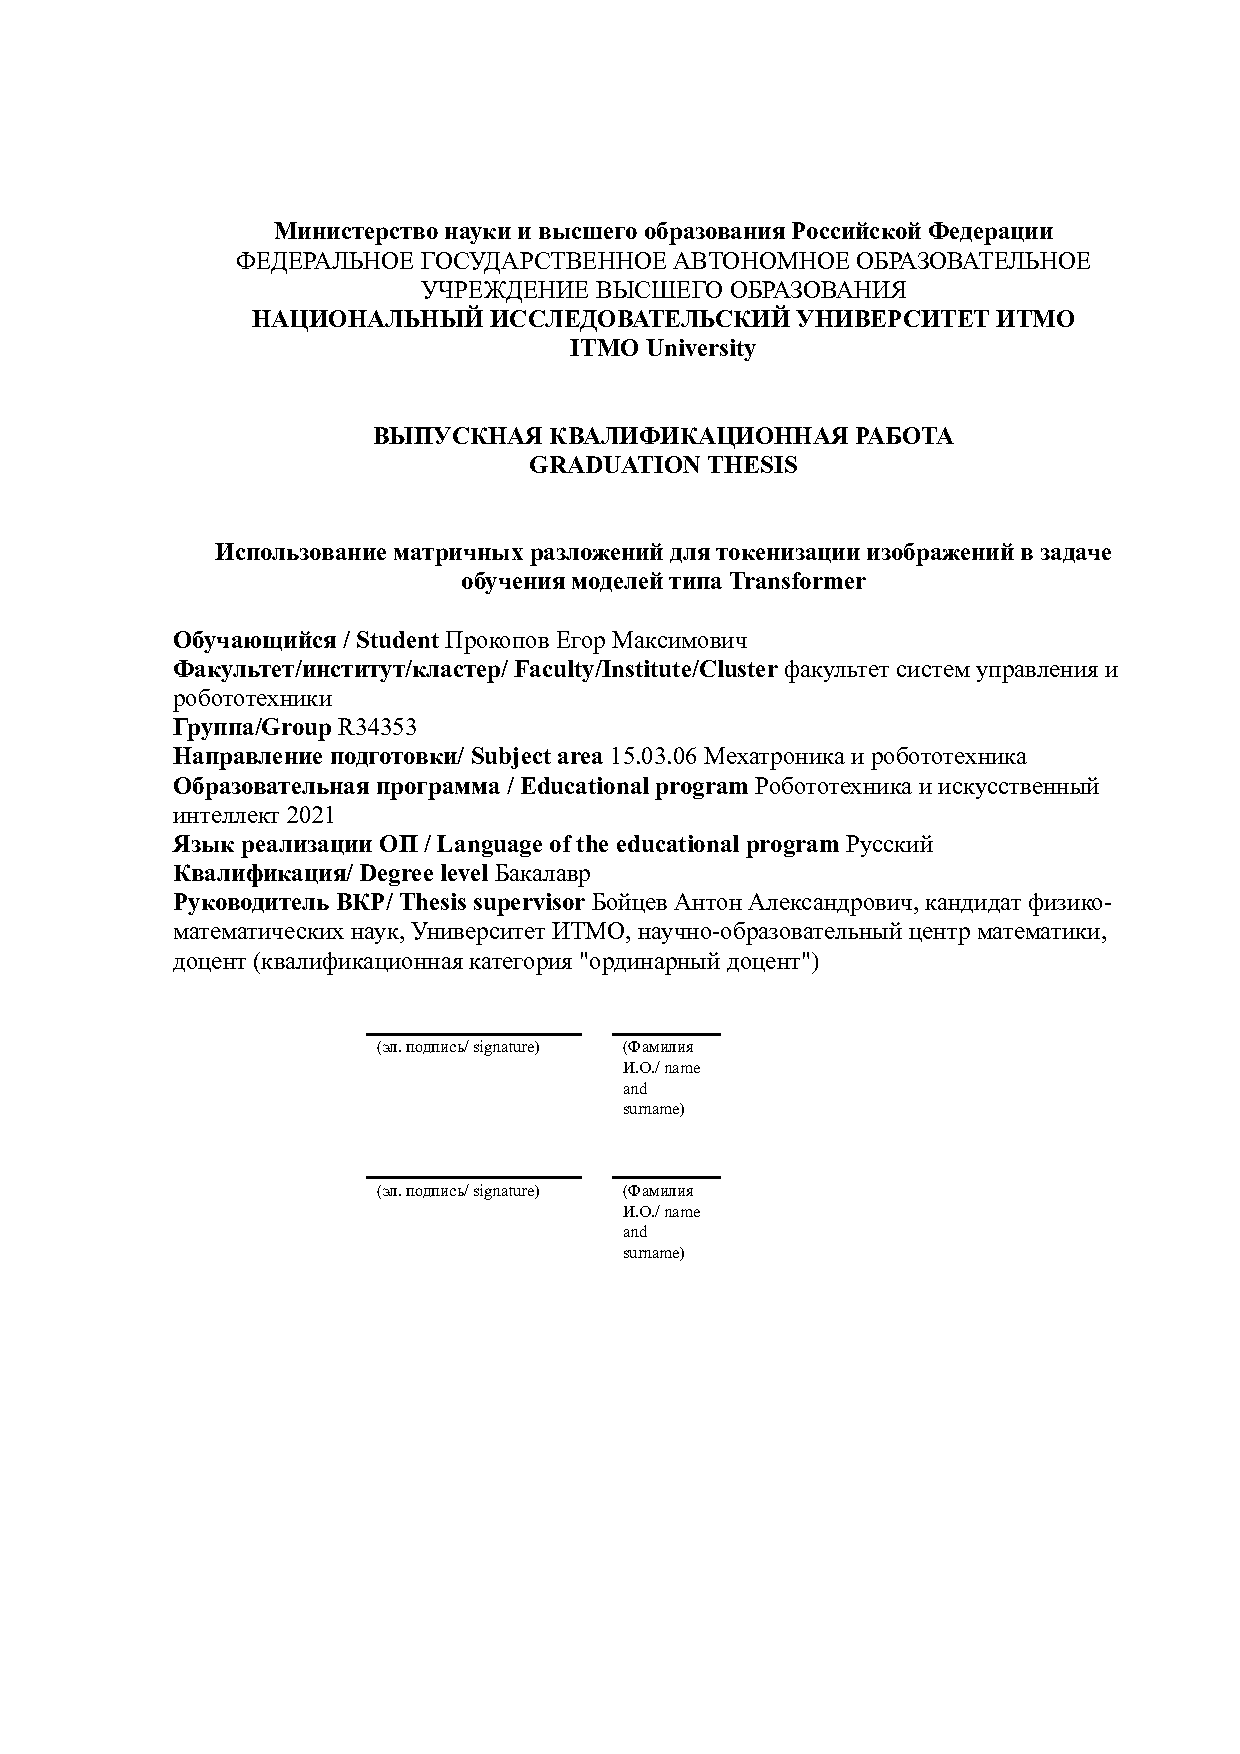
\includepdf[pages=-]{pdfs/tit.pdf}
%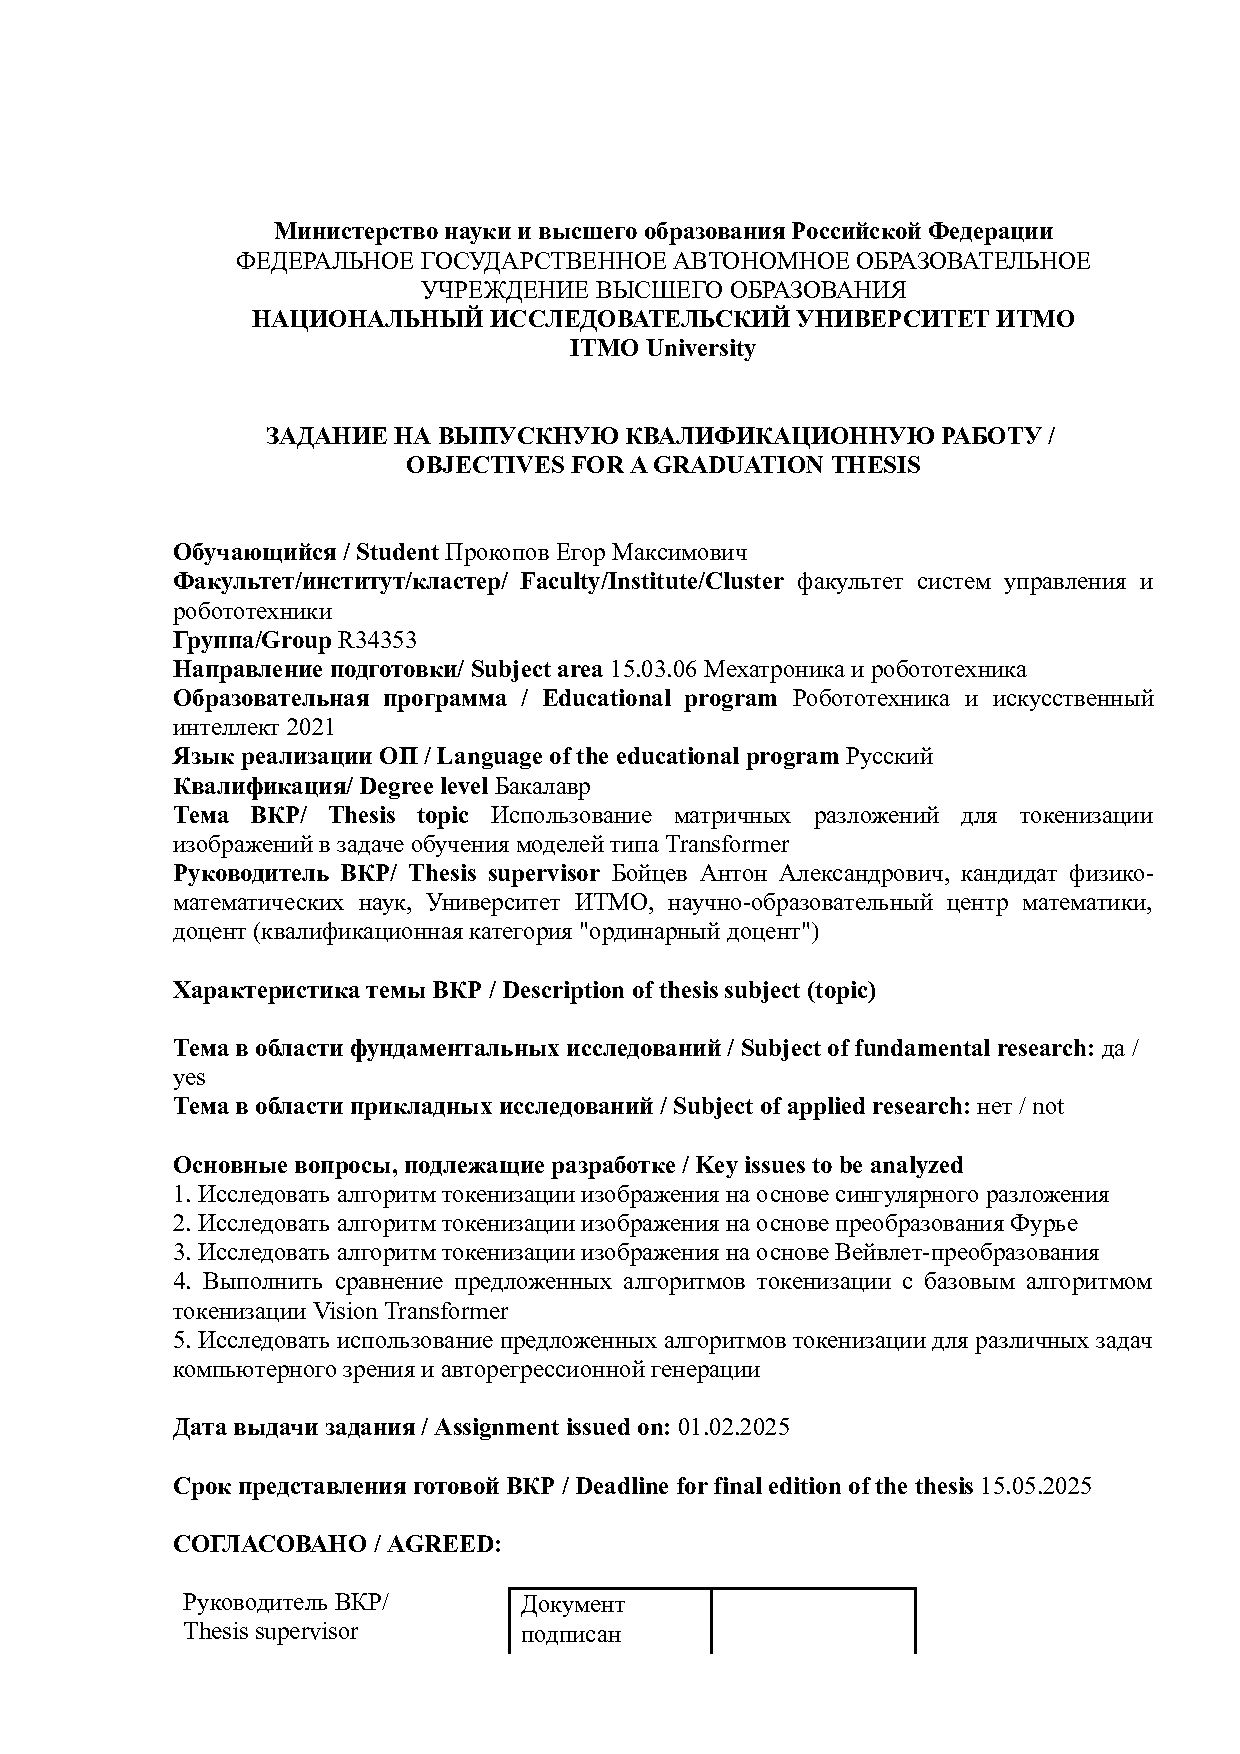
\includepdf[pages=-]{pdfs/Задание_ВКР_Прокопов_Е.М..pdf}
%\includepdf[pages=-]{pdfs/Аннотация__ВКР_Прокопов_Е.М..pdf}


\newpage
\addcontentsline{toc}{section}{Содержание}
\tableofcontents
\newpage
\documentclass[times,specification,annotation]{itmo-student-thesis}
\usepackage{fancyhdr}

%% Опции пакета:
%% - specification - если есть, генерируется задание, иначе не генерируется
%% - annotation - если есть, генерируется аннотация, иначе не генерируется
%% - times - делает все шрифтом Times New Roman, собирается с помощью xelatex
%% - languages={...} - устанавливает перечень используемых языков. По умолчанию это {english,russian}.
%%                     Последний из языков определяет текст основного документа.

%% Делает запятую в формулах более интеллектуальной, например:
%% $1,5x$ будет читаться как полтора икса, а не один запятая пять иксов.
%% Однако если написать $1, 5x$, то все будет как прежде.
\usepackage{icomma}

%% Один из пакетов, позволяющий делать таблицы на всю ширину текста.
\usepackage{tabularx}

%% Данные пакеты необязательны к использованию в бакалаврских/магистерских
%% Они нужны для иллюстративных целей
%% Начало
\usepackage{tikz}
\usetikzlibrary{arrows}
\usepackage{filecontents}
%% Конец

%% Указываем файл с библиографией.
\addbibresource{bachelor-thesis.bib}

\begin{document}

%% Макрос для введения. Совместим со старым стилевиком.
\startprefacepage

В последние годы архитектуры нейронных сетей, основанные на модели Transformer, изначально разработанной для решения задачи машинного перевода, получили широкое распространение. Ключевой механизм данной архитектуры – механизм внимания, который позволяет обрабатывать все элементы входной последовательности параллельно. Такой подход ускоряет обучение при использовании графических ускорителей, значительно улучшает понимание нейронной сетью глобального контекста, а также положительно влияет на масштабируемость системы, позволяя более эффективно обучать нейронные сети с большим числом параметров и на больших наборах данных.  Проблемой механизма внимания является вычислительная сложность и требуемая память $O(n^2 )$, где $n$ – длина входной последовательности.

Изначально модели типа Transformer применялись исключительно для обработки последовательных данных, в основном текста. Однако с появлением модели Vision Transformer (ViT),  стало возможным их применение для решения задач компьютерного зрения.  Архитектурно Vision Transformer повторяет кодировщик оригинальной модели Transformer. Основное отличие заключается в способе преобразования исходных данных в набор векторов. При решении задач обработки естественного языка данный процесс выполняется посредством разбиения единого текста на последовательность частей слов и иных символов – токенов. После каждый токен соотносится с определенным вектором с помощью специальной обучаемой матрицы. Этот процесс называется токенизацией. В Vision Transformer она реализуется через разбиение изображения на фиксированные по размеру части – патчи (чаще всего, 16 на 16 пикселей). После этого, каждый патч выпрямляется в вектор и проецируется в пространство определенной размерности.

Базовый метод токенизации изображений Vision Transformer, хотя и прост в реализации, имеет существенные ограничения. Во-первых, фиксированный размер патчей приводит к избыточной длине входной последовательности, что может быть критичным при обработке изображений высокого разрешения или нескольких изображений одновременно. Во-вторых, статичная сетка разбиения игнорирует структуры объектов на изображении  и их семантическую важность, а также негативно сказывается на понимании нейронной сетью локального контекста. Эти ограничения делают актуальным поиск альтернативных методов токенизации, которые сохранят преимущества моделей Transformer, но при этом обеспечат гибкость и вычислительную эффективность.

В данной работе исследуется применение матричных разложений для создания адаптивного подхода преобразования изображений в последовательность токенов. Данный подход должен позволить уменьшить длину входной последовательности (длину контекста) без потери критически важной информации, а также сохранить или улучшить способность модели к пониманию как глобальных, так и локальных визуальных признаков. 

Основная идея – использовать матричные разложения для получения матриц меньшего порядка. В частности, рассматриваются такие методы как:

\begin{enumerate}
    \item Сингулярное разложение – разложение матрицы прямоугольной формы в произведение трех матриц: левых сингулярных векторов, диагональной матрицы сингулярных чисел и правых сингулярных векторов. По теореме Эккарта-Янга, наилучшая матрица для приближения заданной матрицы с заранее заданным рангом получается из сингулярного разложения исходной матрицы. Таким образом, возможно значительно сократить длину контекста, пожертвовав малой долей информации изображения.
    \item Преобразование Фурье – преобразование, при котором сигнал (изображение в частности) раскладывается на гармонические составляющие. Данный метод позволяет уменьшить длину входной последовательности, пожертвовав малоинформативными высокочастотными признаками.
\end{enumerate}

Для оценки качества работы, рассмотренные методы токенизации сравниваются с базовым методом токенизации ViT на задаче классификации изображений. Также, для общей оценки методов, рассматривается их применение в других задачах, в том числе и авторегрессионной генерации изображений.


\end{document}
\newpage
\section{Анализ предметной области}
\subsection{Архитектура Transformer}

Архитектура Transformer\cite{transformer} (трансформер) стала прорывом в области обработки естественного языка. В отличие от более ранних работ, комбинировавших механизм внимания, сверточные и рекуррентные методы \cite{lstm_cnn_attention_model}, архитектура трансформер избегает использования механизма рекуррентности и основана на использовании только механизма внимания.


\begin{figure}[H]
    \centering
    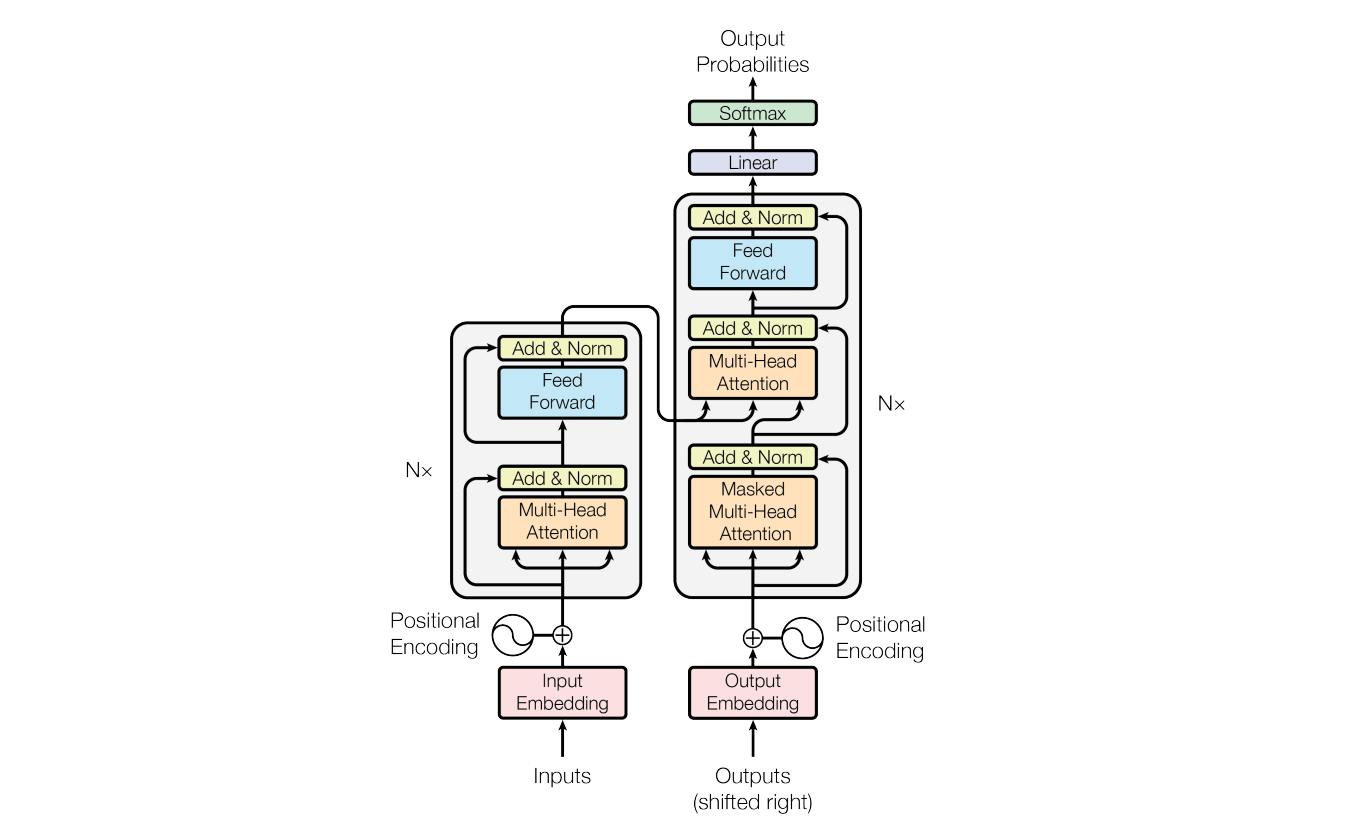
\includegraphics[width=1.0\textwidth]
    {images/domain_analysis/transformer_scheme.png}
    \caption{Схема архитектуры трансформера, взятая из оригинальной статьи.}
    \label{fig:transformer-scheme}
\end{figure}


Трансформер состоит из двух главных блоков (\autoref{fig:transformer-scheme}): трансформер кодировщик и трансформер декодировщик. Трансформер-кодировщик преобразует элементы входной последовательности в последовательность векторов той же длины. Каждый элемент последовательности учитывает связь со всеми остальными элементами, что обеспечивается механизмом внимания. В некоторых моделях, основанных на архитектуре трансформера-кодировщика, например BERT\cite{bert}, к последовательности входных данных добавляется элемент ``CLS``, токен класса. Данный элемент служит для агрегации всей информации последовательности в один плотный вектор.

Трансформер-декодировщик используется для генерации выходной последовательности авторегрессионно, то есть пошагово. В этом режиме, за один шаг работы модели предсказывается один новый элемент на основе предыдущих. 

Для получения последовательности элементов из единого текста применяются методы токенизации. В ходе токенизации, текст разбивается на лексемы, кодируемые при помощи словаря в плотные векторы - токены (слово ``token`` в переводе с английского языка означает ``лексема``, однако поскольку термин ``токен`` в контексте моделей-трансформеров также означает плотный вектор обрабатываемой последовательности, далее он будет использоваться именно в этом смысле).

\subsection{Механизм внимания}

Основа модели трансформер - механизм внимания. В моделях, основанных на архитектуре трансформер-кодировщик, используются механизмы самовнимания и многоглавого внимания. 

Механизм самовнимания вычисляет взаимное влияние элементов последовательности с помощью вычисления матрицы весов. С помощью матриц проекции $W_Q$, $W_K$, $W_V$ для векторов $X$ последовательности вычисляются матрицы ``запросов`` $q$, ``ключей`` $k$ и ``значений`` $v$:

$$
Q = X W_Q, \quad K = X W_K, \quad V = X W_V 
$$

Внимание вычисляется по следующей формуле:

$$
\text{Attention}(Q, K, V) = \text{softmax}\Big(\dfrac{QK^T}{\sqrt{\dim(K_0)}}\Big)V,
$$

где:

$$
\text{softmax}(x_i) = \dfrac{\exp(x_i)}{\sum\limits_{j=0}^{\dim(x)}\exp(x_j)}
$$

Таким образом, за счет вычисления квадратной матрицы весов внимания 

$$\text{softmax}\Big(\dfrac{QK^T}{\sqrt{\dim(K_0)}}\Big)$$

с размерностью, равной длине последовательности, каждый токен последовательности получает информацию о всех остальных токенах.

В многоглавом внимании механизм самовнимания разделяется на $h$ ``голов``, каждая из которых работает в подпространстве меньшей размерности:

$$
\text{MultiHead}(Q, K, V) = \text{Concat}(\text{head}_1, \cdots, \text{head}_h)W^O,
$$

где: 
\begin{itemize}
    \item $W^O$ - матрица проекции,
    \item $\text{head}_i = \text{Attention}(Q W_i^Q, K W_i^K, V W_i^V)$, а $W_i^Q$, $W_i^K$, $W_i^V$ - матрицы проекций в пространство меньшей размерности.
\end{itemize}

При использовании механизма многоглавого внимания, каждая ``голова`` фокусируется на разных аспектах данных параллельно, что позволяет моделировать более сложные зависимости.

\subsection{Применение модели типа Transformer для обработки изображений}

Изначально модели транформер применялись исключительно для обработки последовательных данных. Однако, поскольку данная архитектура обрабатывает каждый элемент параллельно, для обработки других типов данных их необходимо преобразовать в некоторое множество объектов. 

Наивный подход использования механизма самовнимания при обработке изображений подразумевает попиксельную токенизацию изображения. Для изображений большой размерности данный способ может привести к слишком большому размеру входной последовательности. Решение данной проблемы было предложено в работе Image Transformer \cite{image_transformer}, основанное на применении механизма внимания локально для разных групп пикселей. Однако такой подход исключает глобальное внимание.

С появлением Vision Transformer (ViT) \cite{vit} стало возможным эффективное применение моделей трансформеров для решения задач компьютерного зрения. 


\begin{figure}[H]
    \centering
    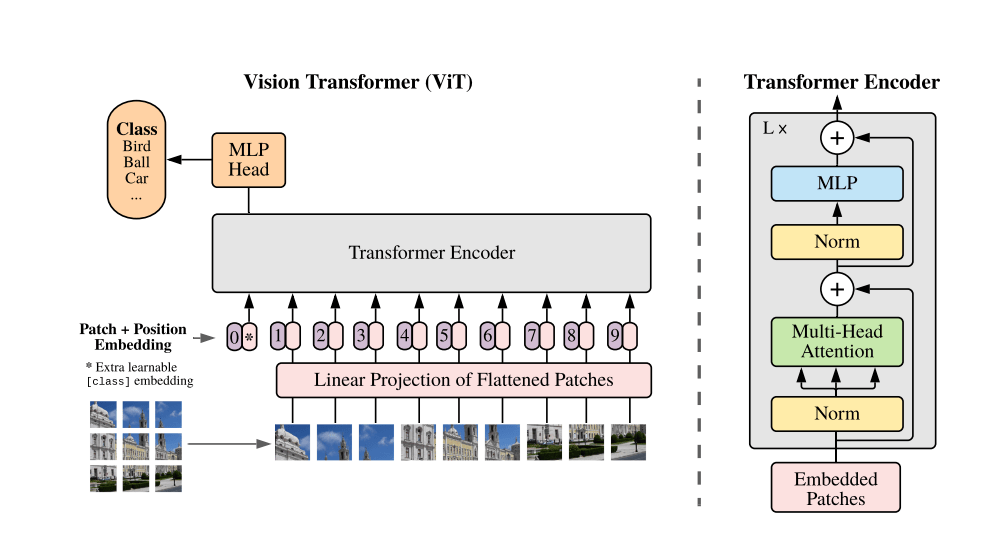
\includegraphics[width=1.0\textwidth]
    {images/domain_analysis/vit_scheme.png}
    \caption{Схема архитектуры Vision Transformer, взятая из оригинальной статьи.}
    \label{fig:vit-scheme}
\end{figure}


Модель ViT повторяет архитектуру (\autoref{fig:vit-scheme}) трансформера-кодировщика, однако заменяет процесс токенизации. В Vision Transformer токенизация реализуется посредством разбиения входного изображения на фиксированные по размеру и непересекающиеся между собой части - патчи (чаще всего, размером 16 на 16 пикселей). После разбиения, каждый патч выпрямляется в вектор и проецируется в пространство определенной размерности. 

Поскольку под термином ``токен`` рассматривается плотный вектор обрабатываемой последовательности, под термином ``токенизация`` будет далее подразумеваться процесс преобразования исходных данных в набор (множество) плотных векторов.

\subsection{Преимущества архитектуры Transformer}

Модели архитектуры трансформер обладают значительными преимуществами перед другими архитектурами:

\begin{itemize}
    \item В отличие от сверточных нейронных сетей, которые обрабатывают локальные паттерны, трансформеры анализируют глобальные зависимости через механизм самовнимания \cite{transformer}.
    \item Архитектура трансформер адаптирована для параллельных вычислений на графических ускорителях \cite{transformer}.
    \item Увеличение количества параметров модели позволяет значительно улучшить качество моделей \cite{gpt2}.
\end{itemize}

\subsection{Недостатки архитектуры Transformer}

Однако, несмотря на все свои преимущества, модель Transformer обладает значительным недостатком. Из-за размерности матрицы весов внимания, вычислительная сложность, а также требуемая память квадратично зависят от длины последовательности \cite{transformer_computation_complexity}.

Эта проблема также касается и обработки изображений. При обработке изображений большой размерности необходимо обрабатывать последовательности большой длины.

\subsection{Выводы по главе 1}
Архитектура трансформер, изначально разработанная для решения задач обработки естественного языка, была успешно адаптирована для обработки изображений благодаря Vision Transformer. Это позволило использовать преимущества модели транформер для обработки изображений. Однако ключевые проблемы трансформеров — квадратичная сложность вычислений механизма самовнимания и квадратичная память не были решены. Эти проблемы могут стать критичными при обработке изображений большого разрешения или нескольких изображений одновременно (например, кадров видео).

\newpage
\documentclass[times,specification,annotation]{itmo-student-thesis}
\usepackage{fancyhdr}

%% Опции пакета:
%% - specification - если есть, генерируется задание, иначе не генерируется
%% - annotation - если есть, генерируется аннотация, иначе не генерируется
%% - times - делает все шрифтом Times New Roman, собирается с помощью xelatex
%% - languages={...} - устанавливает перечень используемых языков. По умолчанию это {english,russian}.
%%                     Последний из языков определяет текст основного документа.

%% Делает запятую в формулах более интеллектуальной, например:
%% $1,5x$ будет читаться как полтора икса, а не один запятая пять иксов.
%% Однако если написать $1, 5x$, то все будет как прежде.
\usepackage{icomma}

%% Один из пакетов, позволяющий делать таблицы на всю ширину текста.
\usepackage{tabularx}

%% Данные пакеты необязательны к использованию в бакалаврских/магистерских
%% Они нужны для иллюстративных целей
%% Начало
\usepackage{tikz}
\usetikzlibrary{arrows}
\usepackage{filecontents}
%% Конец

%% Указываем файл с библиографией.
\addbibresource{bachelor-thesis.bib}

\begin{document}

\chapter{Анализ существующих решений}
Существуют различные методы токенизации изображения (то есть преобразования его в набор плотных векторов).

\section{Токенизация изображений Vision Transformer}
Процесс токенизации изображений в Vision Transformer подразумевает разбиение изображения на патчи.

Данный подход обладает своими преимуществами и недостатками.

\begin{itemize}
    \item По сравнению с методом попиксельной токенизации, предложенной в Image Tranformer, использование патчей вместо пикселей позволяет сократить длину входной последовательности в $s_p^2$ раз при условии разбиения на патчи размером $(s_p, s_p)$. Например, для изображения $(224, 224)$ пикселей, количество элементов входной последовательности снижается с $224^2 = 50 176$ до $ \Big(\dfrac{224}{16}\Big)^2 = 196$.
    \item Поскольку процесс разбиения изображения на патчи $(s_p, s_p)$ с последующей проекцией в пространство некоторой внутренней размерности трансформера можно заменить одним сверточным слоем с размером ядра свертки $s_p$ и шагом $s_p$, можно говорить о сохранении информации о простейших локальных структурах (например, о границах объектов и их текстурах) внутри одного патча.
    \item Поскольку архитектура ViT почти полностью повторяет архитектуру трансформера-кодировщика, токены выходной последовательности могут быть совместимы с текстовыми токенами после, например, линейной проекции или даже без нее. Данное свойство очень важно, поскольку используется в визуальных языковых моделях (VLM), например, в модели LLaVA\cite{llava}, и в таких моделях, как CLIP\cite{clip}, и позволяет связать текстовую модальность и модальность изображений при помощи общей архитектуры трансформера.
\end{itemize}

Однако, несмотря на ряд преимуществ, этот метод токенизации несовершенен. Некоторые из недостатков могут быть критическими при разработке современных моделей. Например, при разработке визуальных языковых моделей, где ставятся высокие требования к длине входной последовательности. Данный метод токенизации имеет следующие недостатки:

\begin{itemize}
    \item Несмотря на сокращение длины входной последовательности в $p_s^2$ раз по сравнению с попиксельной токенизацией, количество патчей, а соответственно токенов, все еще линейно зависит от количества пикселей изображения. Это значит, что при линейном увеличении размера изображения, количество требуемых ресурсов будет расти квадратично. Это может быть критичным при обработке изображений большой размерности, нескольких изображений одновременно (для учета общего контекста этих изображений) или обработки видео.

    \item Поскольку сетка разбиения на патчи фиксирована, наиболее вероятно, что она будет ``разрезать`` объекты, проходя через их границы. В работе \cite{vit_patch_lack} прямо указано, что классическая токенизация Vision Transformer приводит к уничтожению семантики объектов. Из-за этого происходит потеря локальной целостности различных объектов. Например, лицо человека, попавшее на стык нескольких патчей, будет обработано фрагментарно. Данная проблема негативно влияет на понимание моделью локального контекста.
    
    \item Из-за фиксированного размера патчей, классические модели Vision Transformer плохо адаптируются к изображениям разной размерности. Проблеме адаптации Vision Transformer для обработки изображений разного размера посвящена работа \cite{vitar}.   

    \item Из-за метода токенизации и фиксированной сетки разбиения, однотонные и семантически богатые патчи требуют одинакого количества вычислений на обработку \cite{vit_patch_slimming}. Это приводит к нерациональному использованию ресурсов.
\end{itemize}

\section{Токенизация изображений на уровне субъектов}

Для решения проблемы траты одинаковых ресурсов на обработку однотонных и семантически богатых патчей был предложен метод токенизации изображений на уровне субъобъектов. 

В статье \cite{subobject_tokenization} предложен метод токенизации изображения на основе субобъектов (семантически значимых сегментов изображения). Вместо разбиения изображения на фиксированные патчи, авторы используют модель сегментации DirectSAM, спроектированную ими самостоятельно, для выделения структурно-осмысленных частей объектов. С помощью модели SeqAE, также предложенной в этой работе, эти сегменты преобразуются в плотные векторы.

Авторы заявляют о ускорении обучения при использовании данного метода токенизации. Также они указывают, что в отличие от ViT, длина последовательности зависит не от размера изображения, а от количества объектов на нем. 

Однако это преимущество не имеет смысла, поскольку для работы такого подхода необходимо использовать две дополнительные модели для подготовки токенов, что значительно повышает требуемые ресурсы во время работы. По этой причине, этот подход не будет рассмотрен далее, поскольку из-за своего главного недостатка делает невозможным решение задачи уменьшения требуемых для работы модели-трансформера ресурсов.

\section{Токенизация изображений на основе Вейвлет-разложения}

Вейвлет-преобразование --- это инструмент для анализа изображений и сигналов. Данное преобразование выполняет разложение изображения на низкочастотную и высокочастотные составляющие. При этом, низкочастотная составляющая сохраняет большую часть информации изображения. При каждом таком преобразовании требуемый для хранения изображения объем памяти уменьшается \cite{mallat_wavelet}.

В статье \cite{wavelet_tokenization} предложен алгоритм токенизации изображений на основе Вейвлет-разложения:

\begin{itemize}
    \item Выполняется преобразование RBG в YCbCr.
    \item Над полученным изображением в YCbCr формате выполняется Вейвлет-преобразование. Изображение разбивается на уровни детализации (LL, LH, HL и HH). Каждый уровень соответствует разным частотным компонентам.
    \item Малозначимые высокочастотные элементы обнуляются. Это позволяет сократить объем данных без существенной потери информации.
    \item Оставшиеся составляющие объединяются в тензор $W$, в котором каждый вектор соответствует локальной области пикселей.
    \item Векторы тензора $W$ из пиксельного пространства с помощью линейной проекции проецируются в пространство меньшей размерности 
    $$
    E = W Q,
    $$
    где $Q$ - матрица проекции, а $E$ --- проекция $W$ в ``семантическое`` пространство.
\end{itemize}

К преимуществам данного подхода можно отнести:

\begin{itemize}
    \item Возможность настройки детализации изображения перед его обработкой. Это позволяет значительно уменьшить длину входной последовательности и работать даже с изображениями в сверхвысоком ($N > 2048$) качестве.
    \item Устойчивость к адверсариальным атакам. Поскольку малозначимые высокочастотные составляющие обнуляются, значительно снижается влияние шумов.
    \item За счет неоднородности в высокочастотных составляющих модель фокусируется на информативных областях, пропуская малоинформативные.
\end{itemize}

Однако, у данного подхода также есть много проблем:

\begin{itemize}
    \item Зависимость производительности от гиперпараметров (таких как уровень детализации и порог округления высокочастотных признаков). Неверный выбор гиперпараметров может привести к потере слишком важных деталей или недостаточному сжатию. Таким образом для настройки гиперпараметров требуется трудоемкая работа.
    \item Вейвлет-ядра фиксированы и не способны подстраиваться под данные, что уменьшает адаптивность модели.
    \item Многократное вейвлет-преобразование требует дополнительных ресурсов.
\end{itemize}

Несмотря на имеющиеся проблемы, методы токенизации на основе Вейвлет-преобразования получают все большее распространение. В работе \cite{wavelet_autoregression} даже предложен способ авторегрессионной генерации моделью-трансформером на основе вейвлет-разложения. 

\s\chapterconclusion
Несмотря на появление новых методов, область токенизации изображений все еще требует тчательного изучения, поскольку предлагаемые методы все еще не способны побороть алгоритм токенизации, основанный на разбиении изображений на патчи. Метод токенизации на основе Вейвлет-разложения хоть и может быть адаптирован для других задач, однако изначально предназначен только для генерации изображений, а метод токенизации изображений на основе субъектов применим в очень редких случаях, поскольку требует для своей работы две дополнительные модели с большим количеством параметров, что значительно повышает требуемые для работы алгоритма ресурсы. 

\end{document}
\newpage
\section{Исследование алгоритмов токенизации изображений на основе матричных разложений}

Для создания способа токенизации, способного решить проблемы существующих методов, возможно использование различных алгоритмов преобразования и разложения матриц. В этой главе представлено исследование таких методов, как сингулярное разложение и преобразование Фурье, а также сравнение построенных алгоритмов с существующими.

\subsection{Построение инфраструктуры для исследования алгоритмов токенизации на основе матричных разложений}

Для проверки гипотезы о работоспособности построенных токенизаторов решалась задача многоклассовой классификации изображений. Набор данных, используемый для обучения - Intel Image Classification Dataset \cite{intel_image_dataset}, представленных 17 тысячами изображений 6 классов: ``buildings`` (``здания``), ``forest`` (``лес``), ``glacier`` (``ледник``), ``mountain`` (``гора``), ``sea`` (``море``), ``street`` (``улица``). Примеры изображений из набора данных представлены на  \autoref{fig:intel-multiclass-all} .Набор данных состоит из семантически разнообразных и сбалансированных классов. Исходная выборка разбита на тренировочную выборку, состоящую из приблизительно 14 тысяч изображений, и на валидационную, состоящую из 3 тысяч изображений.


\begin{figure}[htbp]
  \centering
  % Первая строка
  \begin{subfigure}[b]{0.3\textwidth}
    \centering
    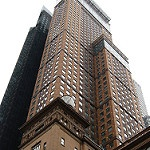
\includegraphics[width=\textwidth]{images/research/dataset/buildings.jpg}
    \caption{``buildings`` (``здания``)}
    \label{fig:intel-multiclass-buildings}
  \end{subfigure}
  \hfill
  \begin{subfigure}[b]{0.3\textwidth}
    \centering
    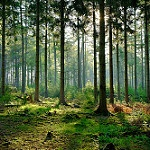
\includegraphics[width=\textwidth]{images/research/dataset/forest.jpg}
    \caption{``forest`` (``лес``)}
    \label{fig:intel-multiclass-forest}
  \end{subfigure}
  \hfill
  \begin{subfigure}[b]{0.3\textwidth}
    \centering
    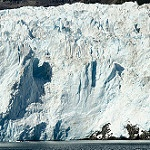
\includegraphics[width=\textwidth]{images/research/dataset/glacier.jpg}
    \caption{``glacier`` (``ледник``)}
    \label{fig:intel-multiclass-glacier}
  \end{subfigure}

  \bigskip % или \\ для переноса

  % Вторая строка
  \begin{subfigure}[b]{0.3\textwidth}
    \centering
    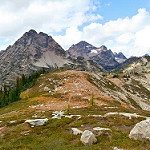
\includegraphics[width=\textwidth]{images/research/dataset/mountain.jpg}
    \caption{``mountain`` (``гора``)}
    \label{fig:intel-multiclass-mountain}
  \end{subfigure}
  \begin{subfigure}[b]{0.3\textwidth}
    \centering
    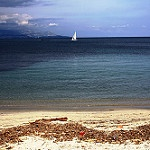
\includegraphics[width=\textwidth]{images/research/dataset/sea.jpg}
    \caption{``sea`` (``море``)}
    \label{fig:intel-multiclass-sea}
  \end{subfigure}
  \hfill
  \begin{subfigure}[b]{0.3\textwidth}
    \centering
    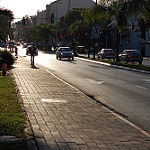
\includegraphics[width=\textwidth]{images/research/dataset/street.jpg}
    \caption{``street`` (``улица``)}
    \label{fig:intel-multiclass-street}
  \end{subfigure}

  \caption{Примеры изображений, представленных в используемом наборе данных}
  \label{fig:intel-multiclass-all}
\end{figure}


Все изображения считываются как трехканальные и масштабируются до размера 256, после чего нормализуются со следующими значениями среднего и стандартного отклонения \cite{torchvision_normalization}: 

$$
\mu = (0.485, 0.456, 0.406), \quad \sigma = (0.229, 0.224, 0.225)
$$

Для реализации предобработки данных изображений использовалась библиотека \texttt{torchvision.transforms}. Для избежания переобучения, использовалась случайная аугментация изображений, а именно:

\begin{itemize}
    \item Случайное обрезание до $0.8$ от размера изначального изображения,
    \item Случайный вертикальная симметрия изображения с вероятностью 0.5
\end{itemize}

При использовании моделей, требующих разбиения изображения на патчи, используется квадратный патч размером 16.

В качестве основной модели, используемой для извлечения и обработки признаков в токен класса используется модель Transformer со следующими параметрами архитектуры:

\begin{itemize}
    \item Размерность токена: 768,
    \item Количество слоев трансформера: 12,
    \item Количество голов внимания трансформера: 12,
    \item Скрытая размерность многослойного перцетрона внутри трансформера: 3072
\end{itemize}

Для классификации изображения по одному из представленных в наборе данных классу используется классификационная голова на основе многослойного перцептрона. Данный модуль на вход принимает значение токена класса. 

Многослойный перцептрон состоит из следующих слоев:

\begin{itemize}
    \item Линейный полносвязный слой с количеством входов, равным размерности токенов трансформера, и 128 выходами,
    \item Функция активации ReLU \cite{relu},
    \item Линейный полносвязный слой с количеством входов 128 и количеством выходов 6
\end{itemize}

Итоговая модель преобразует предобработанное изображение, используя следующую последовательность модулей:

\begin{itemize}
    \item Токенизатор изображения
    \item Модель трансформер
    \item Классификационная голова
\end{itemize}


% Нужна схема

Для построения модели и ее обучения использовались библиотеки  \texttt{torch} и \texttt{lightning.torch}.

Для обучения модели задачи многоклассовой классификации применяется функция потерь перекрестной энтропии \cite{goodfellow_dl}: 

$$
\mathcal{L}_{\mathrm{CE}}
= -\frac{1}{N} \sum_{i=1}^{N} \sum_{c=1}^{C} y_{i,c} \,\log\bigl(\hat{p}_{i,c}\bigr),
$$

где: 

\begin{itemize}
  \item $N$ — число объектов в минибатче,
  \item $C$ — число классов,
  \item $y_{i,c}\in\{0,1\}$ — индикатор того, что $i$-й образец относится к классу $c$,
  \item $\hat{p}_{i,c}=\dfrac{e^{(z_{i,c})}}{\sum_{j=1}^Ce^{(z_{i,j})}}$ — предсказанная моделью вероятность класса $c$ для образца $i$ (применяется функция softmax по выходам $z_{i,*}$).
\end{itemize}

При обучении были применены следующие гиперпараметры:

\begin{itemize}
    \item Размер тренировочного батча: 12
    \item Скорость обучения: 0.0001
    \item Количество эпох: 20
\end{itemize}


Для отслеживания качества обучения модели рассматривались такие метрики, как точность

$$
\text{Accuracy} = \frac{TP + TN}{TP + TN + FP + FN}
$$

и $F_1$-метрика

$$
F_\beta = (1 + \beta^2)\,\frac{\mathrm{Precision}\;\cdot\;\mathrm{Recall}}{\beta^2\,\mathrm{Precision} + \mathrm{Recall}}, \qquad  F_1 = 2 \cdot \frac{\text{Precision} \;\cdot\; \text{Recall}}{\text{Precision} + \text{Recall}},
$$

где:

\begin{itemize}
  \item $TP$ (True Positive) — число объектов положительного класса, правильно отнесённых к положительному классу.
  \item $TN$ (True Negative) — число объектов отрицательного класса, правильно отнесённых к отрицательному классу.
  \item $FP$ (False Positive) — число объектов отрицательного класса, ошибочно отнесённых к положительному классу.
  \item $FN$ (False Negative) — число объектов положительного класса, ошибочно отнесённых к отрицательному классу.
  \item $\text{Precision}$ (точность) — доля правильно классифицированных положительных объектов среди всех объектов, отнесённых к положительному классу

    $$
    \text{Precision} = \frac{TP}{TP + FP}.
    $$
  
  \item $\text{Recall}$ (полнота) — доля правильно классифицированных положительных объектов среди всех действительно положительных объектов

    $$
    \text{Recall} = \frac{TP}{TP + FN}.
    $$
\end{itemize}

Для всех дальнейших экспериментов была применена данная инфраструктура обучения моделей и измерения метрик на валидационной выборке.


\subsection{Токенизация изображений на основе быстрого преобразования Фурье}

\subsubsection{Анализ применения быстрого преобразования Фурье для токенизации изображений}

Рассмотрим черно-белое изображение $i(x, y)$ размера $(M, M)$. Двумерное дискретное преобразование Фурье \cite{gonzalez_woods} позволяет получить частотное представление изображения $I(u, v)$ как

$$
I(u, v) = \sum_{x=0}^{M-1}\sum_{y=0}^{M-1} i(x, y) e^{-i2\pi\Big(\dfrac{ux}{M} + \dfrac{vx}{M}\Big)}
$$

Поскольку вычислительная сложность алгоритма быстрого преобразования Фурье \cite{fft} составляет $O(M^2 \log(M^2))$ вместо $O((M)^4)$, при этом позволяя получить тот же самый результат, далее будет применяться именно этот алгоритм. 

$I(u, v)$ можно представить как изображение с комплекснозначной интенсивностью пикселей, либо же как двухканальное изображение. Для наглядности визуализации используется спект мощности, определяемый как 

$$
I^{power} = \sqrt{(Re(I))^2 + (Im(I))^2}
$$

Также, поскольку зачастую в спектрах мощностей присутствуют значительные пики (большие значения) малого количества частот, используется масштабирование спектра мощности

$$
\log(I^{power}) \quad \text{или} \quad \sqrt{I^{power}}
$$

В дальнейшем, при вычислении спектра мощности будет использоваться именно метод масштабирования на основе логарифма.

Также стоит отметить, что при визуализации или построении низкочастотного фильтра, используется центрированный спектр мощности. Поскольку в $I^{power}$ низким частотам соответствуют значения на краях, для удобства последующей обработки применяется центральная симметрия.

\subsubsection{Построение низкочастотного фильтра}

Поскольку высокие частоты содержат лишь малую долю информации, можно построить фильтр низких частот \cite{low_pass_filter}, отсекающий высокие частоты. Такой подход позволяет значительно сократить количество обрабатываемых данных при сохранении основной информации, а также позволяет очистить исходное изображение от шумов. Обычно, для построения такого фильтра используется отбор частот с помощью евклидовой расстояния до центра спектра мощности.

\begin{figure}[H]
    \centering
    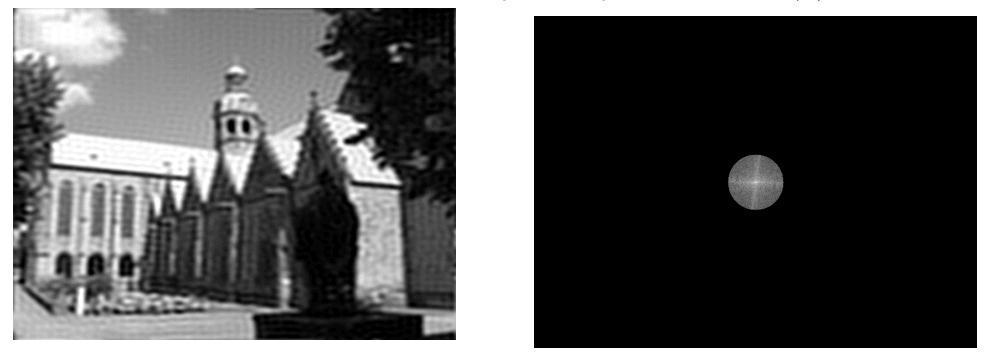
\includegraphics[width=1.0\textwidth]
    {images/solutions_analysis/fourier/low_pass_filter.png}
    \label{fig:svd_approx_im_fix_rank}
    \caption{Фильтр низких частот с использованием евклидова расстояния до центра спектра мощности.}
\end{figure}

В дальнейшем выход низкочастотного фильтра будет обрабатываться нейронной сетью. Однако, так как нейронные сети обрабатывают матрицы, использование конкретно данного фильтра приведет к тому, что в углах выхода низкочастотного фильтра будут находиться нули. В свою очередь, это приведет к лишним вычислениям и затратам памяти, не улучшающих итоговый результат работы модели. Также, это сократит объем полезной информации, используемой трансформером для обработки. Поэтому, для того, чтобы сохранить больше полезной информации, выполним отбор частот не с помощью расстояния Евклида

$$
d_{\mathrm{E}}(\mathbf{x}, \mathbf{y})
= \sqrt{\sum_{i=1}^{n} (x_i - y_i)^2},
$$

а с помощью расстояния Чебышева

$$
d_{\mathrm{Ch}}(\mathbf{x}, \mathbf{y})
= \max_{1 \le i \le n} \bigl|x_i - y_i\bigr|.
$$

% нужна картинка низкочастотного фильтра с расстоянием Чебышева

Для обработки многоканальных (в том числе и цветных) изображений, представим их с помощью трёх матриц, к каждой из которых применим быстрое преобразование Фурье и низкочастотный фильтр по одинаковой маске. В результате получим тензор размерности (6, $s$, $s$), где $s$ - размер фильтра, то есть предельное расстояние (с использованием нормы Чебышева), при котором частоты сохраняются в результате отбора низкочастотного фильтра.

\subsubsection{Вычисление размера фильтра}
Размер фильтра может быть задан как фиксированный гиперпараметр. Такой фильтр назовем статическим фильтром.

Однако, в этом случае результат работы модели будет сильно отличаться в зависимости от размера входного изображения. Так, при обработке больших изображений, многократно больших, чем размер фильтра, будут отбираться только самые низкие частоты. В это же время, при обработке изображений, размер которых соответствует размеру фильтра или их размер меньше размера фильтра, будут учитываться абсолютно все частоты. Это делает вычисление размера фильтра важной задачей при построении токенизатора на основе быстрого преобразования Фурье.

Очевидно, что размер фильтра должен коррелировать с размером обрабатываемого изображения. Это делает размер фильтра $s$ динамически изменяемым параметром. Для определения $s$ воспользуемся центрированным отмасштабированным спектром мощности. Можно заметить, что низкие частоты имеют значительно большую интенсивность, чем высокие частоты. Сумму всех интенсивностей назовем энергией спектра мощности 

$$
E = \sum\limits_{i=-M/2}^{M/2}\sum\limits_{j=-M/2}^{M/2} I^{power}(i, j)
$$ 

Поскольку для построения токенизатора нам необходимы в первую очередь низкие частоты, будем увеличивать размер фильтра $s$ таким образом, пока доля охватываемой фильтром энергии спектра мощности не превысит $pE$, где $p \in (0, 1]$ - гиперпараметр, который назовем долей энергии спектра мощности.

Таким образом, значение $s$ можно вычислить с помощью условия

$$
\sum_{i=-s/2}^{s/2}\sum_{j=-s/2}^{s/2} I^{power}(i, j) \leq pE < \sum_{i=-\frac{s+1}{2}}^{\frac{s+1}{2}}\sum_{j=-\frac{s+1}{2}}^{\frac{s+1}{2}} I^{power}(i, j)
$$

Для вычисления значения $s$ в программе используются двумерные кумулятивные суммы.

Такой фильтр, размер которого вычисляется с помощью относительной энергии спектра мощности, назовем динамическим фильтром. 

Статический и динамический фильтры обладают следующими преимуществами и недостатками:

\begin{itemize}
    \item Размер статического фильтра всегда одинаков, соответственно, после токенизации, количество токенов входной последовательности трансформера будет неизменным. Это делает количество требуемых вычислительных ресурсов независимым от размера изображения. В свою очередь размер динамического фильтра зависит от размера входного изображения, что может привести к слишком большой длине входной последовательности при обработке изображений большого размера
    \item В отличие от статического фильтра, динамический фильтр позволяет более гибко отбирать частоты, поскольку размер фильтра зависит от того, что изображено на изображении. Так, если изображение состоит из слабоменяющихся, больших и однотонных элементов, то у такого изображения будут преобладать низкие частоты, а соответственно, размер фильтра будет меньше. Если на изображении преобладают высокие частоты, то размер фильтра будет больше.
\end{itemize}



\subsubsection{Построение токенизатора на основе низкочастотного фильтра}

Для построения токенизатора изображения на основе быстрого преобразования Фурье построим низкочастотный фильтр. Маску низкочастотного фильтра будем формировать на основе нормы Чебышева, поскольку в этом случае маска получается квадратная. В результате, цветное изображение размерности $(3, M, M)$ преобразуется в тензор размерности $(6, s, s)$. 

Были рассмотрены различные способы преобразования этого тензора в последовательность векторов.

Первый из рассмотренных способов - способ разбиения на патчи. Данный способ повторяет метод, предложенный в Vision Transformer, однако разбиение на патчи применяется не напрямую к изображению, а к выходу низкочастотного фильтра.

\begin{figure}[H]
    \centering
    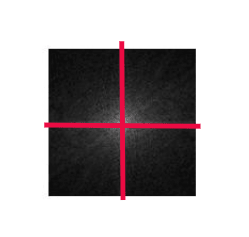
\includegraphics[width=0.5\textwidth]
    {images/research/fourier/patches_split.png}
    \caption{Пример разбиения выхода низкочастотного фильтра на 4 патча.}
\end{figure}

После разбиения на патчи, каждый патч выпрямляется в вектор. Таким образом, тензор размерности 

$$ (6, s, s)$$ 

преобразуется в последовательность векторов размерности 

$$\Big(\dfrac{s^2}{s_p^2}, 6 \cdot s_p^2\Big)$$ 

где $s_p$ - размер одного патча. После этого преобразования каждый вектор полученной последовательности проецируется с помощью линейного полносвязного слоя, называемого слоем проекции, в пространство токенов трансформера. Эта проекция необходима, так как размерность векторов полученной последовательности может не совпадать с требуемой размерностью токенов для обработки их трансформером. 

В программе процесс разбиения изображения на патчи, их выравнивание и линейную проекцию линейным полносвязным слоем можно заменить на свёрточный слой нейронной сети с ядром свертки и шагом свертки равными размеру патча.

К полученной последовательности токенов добавляется токен класса и позиционное кодирование, аналогичное позиционному кодированию в Vision Transformer.

Вторым рассмотренным способом преобразования входного тензора в последовательность векторов является метод интервального разбиения. Результатом применения низкочастотного фильтра является карта признаков, отражающая не пространственные связи между фильтрами, а степень влияния различных частотных компонентов. Метод разбиения на интервалы позволяет сгруппировать эти компоненты по частотным интервалам. Это в свою очередь позволяет модели трансформера в дальнейшем, при обработке входного тензор, выделить наиболее значимые частотные диапазоны. 

\begin{figure}[H]
    \centering
    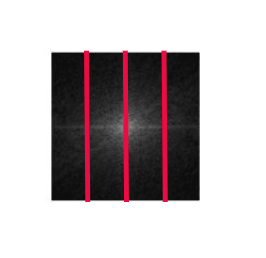
\includegraphics[width=0.5\textwidth]
    {images/research/fourier/bins_split.png}
    \caption{Пример разбиения выхода низкочастотного фильтра на 4 интервала.}
\end{figure}

В этом подходе выход низкочастотного фильтра разбивается на $n_b$ ``полос`` - интервалов. Количество интервалов $n_b$ - гиперпараметр. Каждый такой интервал выпрямляется в вектор. Таким образом, исходный тензор размерности 

$$
(6, s, s) 
$$

преобразуется в последовательность векторов размерности

$$
\Big(n_b, \dfrac{s^2}{n_b}\Big)
$$

Каждый вектор полученной последовательности проецируется с помощью линейного полносвязного слоя в в пространство токенов трансформера. Аналогично методу с разбиением на патчи, эта проекция необходима для приведения полученных векторов к размерности, которую возможность обработать трансформером.

К полученной последовательности токенов добавляется токен класса и позиционное кодирование, аналогичное позиционному кодированию в оригинальной модели Transformer. 

Данный способ разбиения входного тензора на интервалы обладает существенными недостатками. Так, его применение возможно только при использовании статического фильтра низких частот, так как в случае использования динамического фильтра, размер фильтра $s$ - также динамический. Это значит, что последовательность векторов, полученная после разбиения на интервалы выхода низкочастотного фильтра, состоит из векторов динамической размерности $\dfrac{s^2}{n_b}$. Это делает невозможным их проекцию в пространство фиксированной размерности с помощью линейного полносвязного слоя. Данный недостаток существенен, поскольку лишает итоговый токенизатор гибкости при фильтрации токенов.

Поскольку метод разбиения на патчи не обладает недостатками, которыми обладает метод разбиения на интревалы, рассмотрим способы его углубления. Как ранее было отмечено, процесс разбиения изображения на патчи, а при построении токенизатора на основе быстрого преобразования Фурье - выхода низкочастотного фильтра, можно заменить на свёрточный слой с размером свёртки и шагом свертки, равным размеру патча.

Важно отметить, что один свёрточный слой с ядром свёртки размером 5, шагом 1, отступом 1 и без использования нейрона смещения может быть заменен \cite{conv_replace} двумя свёрточными слоями с ядром свёртки размером 3, шагом 1, отступом 1 и также без использования нейрона смещения. В этом случае область, которую обрабатывают эти слои за один шаг остается той же, при этом между двумя свёрточными слоями можно добавить больше функций активации, что позволит итоговой нейронной сети аппроксимировать гораздо более сложные функции. При этом уменьшится количество параметров: при использовании свёрточного слоя с ядром свёртки размером 5, количество параметров на одно ядро становится равным 25, а при использовании двух слоёв с ядром свёртки размером 3, эквивалентное количество параметров равно 18. 

Данный процесс ``разложения`` свёрточных слоёв на свёрточные слои с ядрами свёртки размером 3 можно применить и для свёрточных слоёв с размерами ядер свёртки 15 и 17 (что близко к размеру ядра свёртки 16 - наиболее часто используемому размеру патча). Например, свёрточный слой с размером ядра свёртки 15 можно разложить на последовательность из 7 свёрточных слоёв с размером ядра свёртки 3, а свёрточный слой с размером ядра свёртки 17 можно разложить на 8 свёрточных слоев с размером ядра свёртки 3. 

Однако, в этом случае не получится изменить размер шага свёртки. Из-за этого, после применения такой последовательности свёрточных слоёв с размером ядра свёртки 3, не изменится размер карт признаков. Однако при этом, количество карт признаков увеличится.

Таким образом, исходный тензор размерности

$$(6, s, s)$$

будет преобразован в тензор размерности 

$$
(s_E, s, s),
$$

где $s_E$ - размерность токенов трансформера. Очевидно, что количество обрабатываемых данных вырастет многократно, при этом количество полезной информации нисколько не изменится. 

Для уменьшения размерности карт признаков при обработке изображений свёрточными нейронными сетями часто используют слои объединения (пулинга) \cite{goodfellow_dl}. Эти слои позволяют уменьшить размерность карт признаков, пожертвовав частью информации. Этот подход не удовлетворителен, так как потеря информации приведет к ухудшению качества работы итоговой модели. 

Вместо этого, рассмотрим нейронную сеть Super Resolution Generative Adversarial Network (SRGAN) \cite{srgan}. Это генеративная соревновательная нейронная сеть, созданная специально для решения задачи повышения разрешения изображения. В этой модели, для получения карт признаков большей размерности, используется алгоритм пиксельного перемешивания (pixel shuffle). Данный алгоритм группирует карты признаков по 4, после чего объединяет их в одну карту признаков с размером в 2 раза больше по длине и по ширине. В ходе объединения, элементы с одних и тех же позиций разных карт признаков объединяются в квадраты размером 2 на 2 с сохранением исходных позиций. Данный алгоритм позволяет изменить форму обрабатываемых данных, никак не меняя сами данные.

Поскольку текущая задача противоположная, применим алгоритм пиксельной расстановки (pixel unshuffle) - операцию, обратную алгоритму пиксельного перемешивания. В этом случае одну карту признаков будем разбивать на 4 карты с уменьшением исходной длины и ширины в 2 раза. 

В итоге, для того, чтобы заменить свёрточный слой с ядром свёртки размером 16 и шагом 4, применим после каждого свёрточного слоя c ядром свёртки размером 3 и функции активации алгоритм пиксельной расстановки. Количество таких блоков определяется размером заменяемого патча. В случае с размером патча 16, количество таких блоков равно 4, так как $2^4 = 16$. Поскольку в этом случае от размера выхода низкочастотного фильтра требуется кратность 16, рассчитанный размер фильтра округляется в большую сторону до первого значения, кратного 16.


Таким образом, исходный тензор размерности

$$
(6, s, s)
$$

преобразуется в тензор размерности

$$
\Big(s_E, \dfrac{s}{16}, \dfrac{s}{16}\Big)
$$

Данный тензор выпрямляется по двум последним осям и транспонируется. Следом каждый вектор последовательности проецируется с помощью полносвязного линейного слоя с количеством входов и количеством выходов, равными размерности токена. После этого получается последовательность векторов --- токенов, готовых к обработке моделью трансформер. Такая последовательность имеет форму.

$$
\Big(\dfrac{s^2}{16^2}, s_E\Big)
$$


Итоговая схема изображена на \autoref{fig:mfft-scheme}.

\begin{figure}[H]
    \centering
    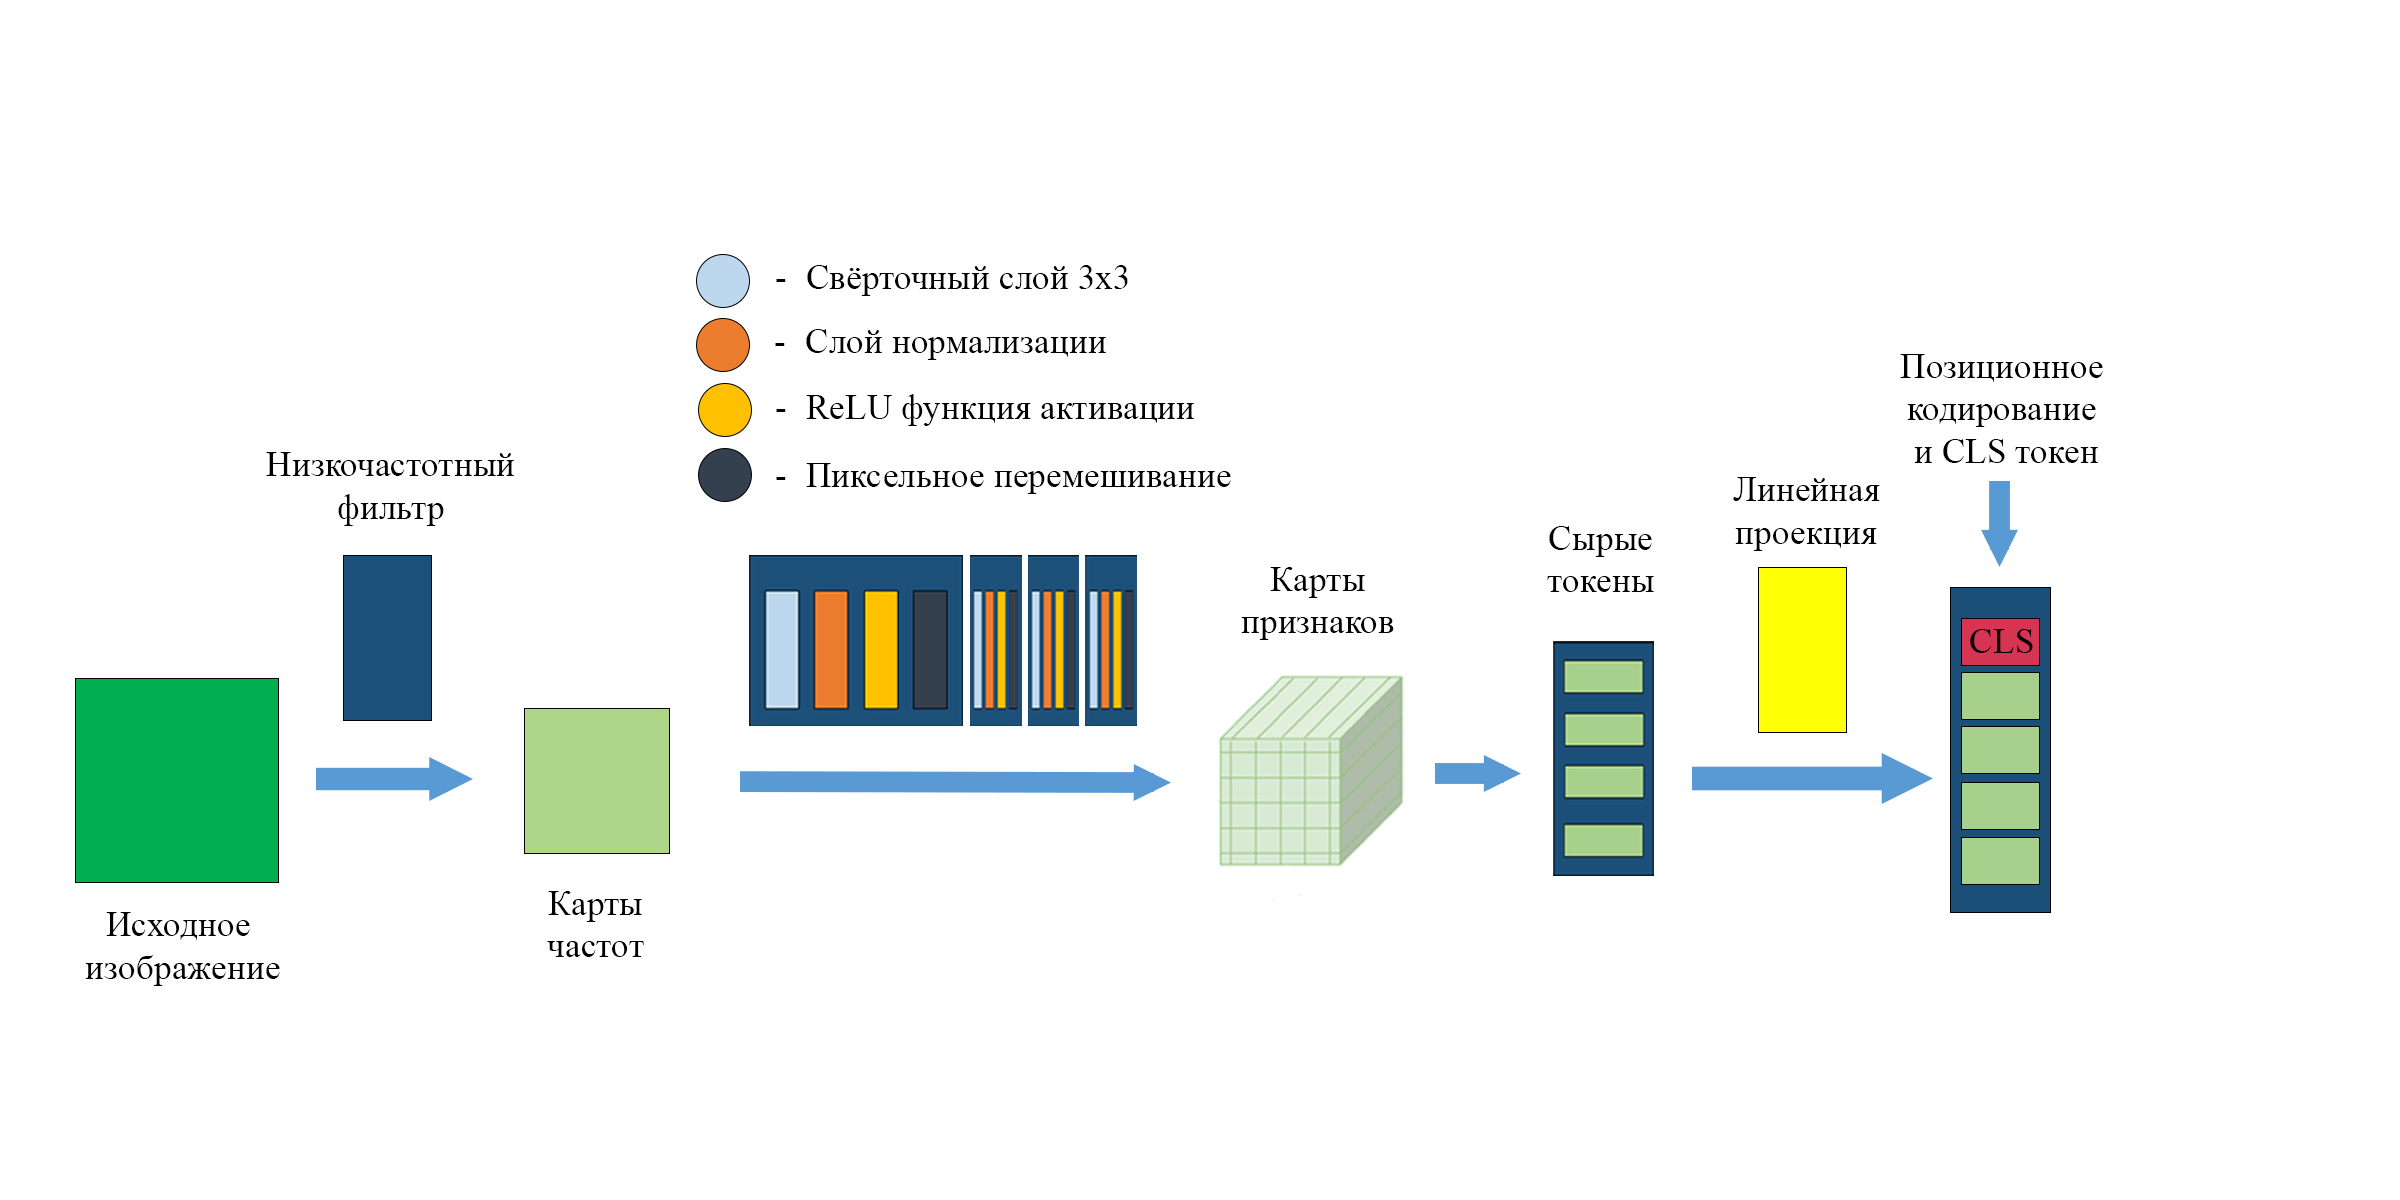
\includegraphics[width=1.0\textwidth]
    {images/research/fourier/mfft_scheme.png}
    \caption{Схема токенизатора на основе быстрого преобразования Фурье.}
    \label{fig:mfft-scheme}
\end{figure}

\subsubsection{Результаты обучения}

Во время обучения моделей с токенизатором на основе быстрого преобразования Фурье не использовалась нормализация изображений кроме отдельно рассмотренного эксперимента.

Было проведено сравнение методов токенизации с использованием быстрого преобразования Фурье. Результаты обучения представлены в \autoref{table:fft-tokenization}.

\begin{table}[H]
  \centering
  \begin{tabular}{|l|c|c|}
    \hline
    Метод токенизации & Точность & $F_1$-метрика \\ \hline
    Vision Transformer & 0.79 & 0.79  \\
    FFT-токенизация (патчи) & 0.16 & 0.16  \\ 
    FFT-токенизация (интервалы)  & 0.17 & 0.17  \\ 
    FFT-токенизация (пиксельное перемешивание) & 0.79 & 0.79 \\
    \hline
  \end{tabular}
    \caption{Сравнение результатов обучения моделей с различными токенизаторами на основе быстрого преобразования Фурье с моделью Vision Transformer.}
  \label{table:fft-tokenization}
\end{table}

Из результатов обучения \autoref{table:fft-tokenization} видно, что из всех рассмотренных методов токенизации, единственным работоспособным оказался только метод токенизации с использованием пиксельного перемешивания. Поэтому следующие эксперименты были проведены только с использованием этого метода.

Далее было проведено сравнение методов токенизации с использованием низкочастотного и высокочастотного фильтров. Был исследован метод токенизации, аналогичный рассмотренному ранее, только с использованием высокочастотного фильтра вместо низкочастотного. Для построения высокочастотного фильтра не применялась центральная симметрия результата работы алгоритма быстрого преобразования Фурье. Было проведено сравнение при различных значениях размера статического фильтра. Результаты обучения и замера метрик представлены в \autoref{tab:fft-tokenization-unshifted}.

\begin{table}[H]
  \centering
  \begin{tabular}{|l|c|c|c|}
    \hline
    Метод токенизации & Размер фильтра & Точность & $F_1$-метрика \\ \hline
    Низкочастотный фильтр & 256 & 0.79 & 0.79 \\
    Высокочастотный фильтр & 64 & 0.32 & 0.25 \\
    Высокочастотный фильтр & 128 & 0.51 & 0.51 \\
    Высокочастотный фильтр & 256 & 0.79 & 0.79 \\
    \hline
  \end{tabular}
    \caption{Сравнение результатов обучения моделей с токенизатором с высокочастотным фильтром при разных размерах фильтра с токенизатором с низкочастотным фильтром.}
  \label{tab:fft-tokenization-unshifted}
\end{table}

Из \autoref{tab:fft-tokenization-unshifted} видно, что низкие частоты оказывают значительное влияние на итоговое качество работы модели, что подтверждает изначальную гипотезу о их важности при обучении нейронной сети. Также можно заметить, что модель с токенизатором с высокочастотным фильтром и малым размером фильтра, несмотря на серьезное падение значений метрик, работоспособна.

Также было выполнено сравнение размеров статического низкочастотного фильтра и проведено исследование их влияния на результат обучения модели. Результаты обучения и замера метрик представлены в \autoref{tab:fft-tokenization-static}.

\begin{table}[H]
  \centering
  \begin{tabular}{|l|c|c|c|}
    \hline
    Метод токенизации & Размер фильтра & Точность & $F_1$-метрика \\ \hline
    Vision Transformer & - & 0.79 & 0.79 \\
    Низкочастотный фильтр & 64 & 0.76 & 0.76 \\
    Низкочастотный фильтр & 128 & 0.78 & 0.78 \\
    Низкочастотный фильтр & 256 & 0.79 & 0.79 \\
    \hline
  \end{tabular}

    \caption{Сравнение результатов обучения моделей с токенизатором с низкочастотным фильтром при разных размерах статического фильтра.}
  \label{tab:fft-tokenization-static}
\end{table}

Из \autoref{tab:fft-tokenization-static} видно, что серьезное уменьшение размера фильтра (в 4 раза) привело к лишь незначительному снижению качества работы модели как по сравнению с моделью с размером фильтра, равным размеру изображения, так и по сравнению с Vision Transformer. Важно также заметить, что уменьшение размера фильтра в 4 раза привело к уменьшению размера входной последовательности токенов для обработки трансформером в 16 раз. 

Далее было проведено исследование влияния сохраняемой доли энергии спетра мощности на обучение модели. Результаты обучения и замера метрик представлены в \autoref{tab:fft-tokenization-dynamic}.

\begin{table}[H]
  \centering
  \begin{tabular}{|l|c|c|c|}
    \hline
    Метод токенизации & Размер фильтра & Точность & $F_1$-метрика \\ \hline
    Vision Transformer & - & 0.79 & 0.79 \\
    Низкочастотный фильтр (0.900) & 96 & 0.74 & 0.74 \\
    Низкочастотный фильтр (0.950) & 128 & 0.76 & 0.76 \\
    Низкочастотный фильтр (0.990) & 208 & 0.77 & 0.76 \\
    \hline
  \end{tabular}

    \caption{Сравнение результатов обучения моделей с токенизатором с низкочастотным фильтром при разных размерах динамического фильтра (значение сохраняемой доли энергии указано в скобках возле названия метода токенизации)}
  \label{tab:fft-tokenization-dynamic}
\end{table}

Из \autoref{tab:fft-tokenization-dynamic} видно, что заметно не сильное падение значений метрик при значительном уменьшении размера фильтра. Также, если сравнивать результаты обучения с использованием динамического фильтра и с использованием статического фильтра, можно заметить, что при одинаковых размерах фильтра, при использовании динамического фильтра значения метрик оказываются немногим ниже, чем при использовании статического фильтра. Вероятно, на это повлияла динамическая длина последовательности при обучении модели.

Также, было важным провести исследование влияния нормализации изображений на работу токенизатора.

Нормализация изображений - простое афинное преобразование, которое приближает значения пикселей к стандартному нормальному распределению и выравнивает статистики RGB-каналов изображения. Данный метод предобработки изображений делает процесс обучения нейронной сети более быстрым, стабильным и надёжным \cite{goodfellow_dl}. Отсутствие нормализации замедляет обучение модели.

Однако, применение нормализации изображений может привести к потери части информации о низких частотах и исказить относительные амплитуды.

Было проведено исследование влияния нормализации изображений на обучение модели с токенизатором на основе быстрого преобразования Фурье. Результаты обучения и замера метрик представлены в \autoref{tab:fft-tokenization-norm}.

\begin{table}[H]
  \centering
  \begin{tabular}{|l|c|c|c|}
    \hline
    Нормализация & Размер фильтра & Точность & $F_1$-метрика \\ \hline
    Присутствует & 128 & 0.48 & 0.48 \\
    Отсутствует & 128 & 0.78 & 0.78 \\
    \hline
  \end{tabular}

    \caption{Сравнение результатов обучения моделей при наличии и отсутствии нормализации изображений во время обучения.}
  \label{tab:fft-tokenization-norm}
\end{table}

Как видно из \autoref{tab:fft-tokenization-norm}, нормализация изображений очень негативно влияет на результаты обучения моделей с использованием токенизатора на основе быстрого преобразования Фурье. Происходит падение точности почти в два раза. Таким образом, можно сделать вывод, что при обучении моделей с использованием данного токенизатора, использование нормализации изображений нежелетельно.

\subsection{Токенизация изображений на основе сингулярного разложения}

\subsubsection{Анализ применения сингулярного разложения для токенизации изображений}

Сингулярное разложение \cite{loginov_svd} матрицы $I$ размерности $(M, N)$ --- разложение вида 

$$
I = U\Sigma V^*,
$$

где $\Sigma$ --- диагональная матрица сингулярных чисел размерности $(M, N)$, $U$ --- матрица размерности $(M, M)$, $V$ - матрица размерности $(N, N)$, а $V^*$ - эрмитово-сопряженная матрица матрицы $V$. Матрицы $U$ и $V$ - матрицы левых и правых сингулярных векторов соответственно. Сингулярные числа неотрицательны. Поскольку рассматривается применение сингулярного разложения только для токенизации изображений, то есть вещественных матриц, то $V^* = V^T$.

Компонентой сингулярного выражения назовем сингулярное число и соответствующие ему левый и правый сингулярные вектора.

По свойствам сингулярного произведения, можно одновременно переставлять соответствующие столбцы матриц $U$ и $V$ вместе с диагональными элементами, не меняя результата произведения. Для дальнейшего удобства, переставим компоненты сингулярного разложения в порядке убывания сингулярных чисел.

\subsubsubsection{Приближение изображения с помощью сингулярного разложения при фиксированном ранге}

По теореме Эккарта-Янга\cite{eckart_young}, если требуется приблизить матрицу $I$ другой матрицей $I_k$ с заранее заданным рангом $k$ (рангом приближения), чтобы значение $||I - I_k||_2^2$ было минимальным, то наилучшая такая матрица получается из сингулярного разложения матрицы $I$ по формуле:

$$
I_k = U_k\Sigma_kV_k^T
$$

где $\Sigma_k$ - матрица $k$ первых (наибольших) сингулярных чисел, а матрицы $U$ и $V$ состоят из соответствующих им сингулярных векторов. Таким образом можно приблизить матрицу $I$ по заданному рангу. 

Представим цветное трехканальное изображение (для упрощения будем рассматривать только квадратные изображения) как набор трех матриц. Тогда, выполнив приближение каждой из этих матриц по выбранному рангу $k$, можно получить приближение исходного изображения.

\begin{figure}[H]
    \centering
    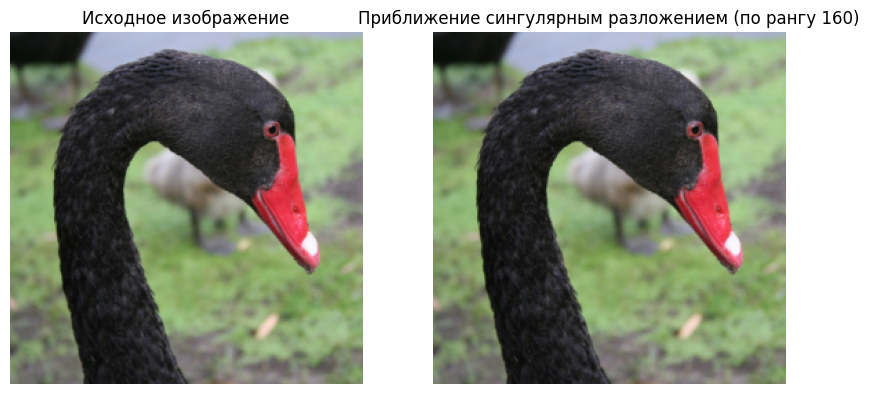
\includegraphics[width=1.0\textwidth]
    {images/solutions_analysis/svd/svd_approx_im_160rank.png}
    \caption{Сравнение исходного изображения (размером 256 на 256 пикселей) и приближения сингулярным разложением по рангу 160.}
    \label{fig:svd-approx-im-fix-rank}
\end{figure}

Из \autoref{fig:svd-approx-im-fix-rank} видно, что при приближении изображения сингулярным разложением нет потери визуальной информации.

При этом, если выбрать сингулярное разложение как основу для токенизации изображений, а компоненты сингулярного разложения представить в виде этих самых токенов, то такое приближение позволит уменьшить длину входной последовательности с 256 до 160.

\subsubsection{Приближение изображения с помощью сингулярного разложения при динамическом ранге}

При решении задачи приближения некоторой матрицы матрицей меньшего ранга с помощью сингулярного разложения, сингулярные значения, возведенные в квадрат, можно интерпретировать как дисперсию, которую ''вкладывает'' в итоговый результат каждая компонента. Причем, чем больше значение сингулярного числа, тем большей части информации оно соответствует. 

Поскольку в общем случае изображения могут сильно отличаться друг от друга, и в одном примере для сохранения большей части информации потребуется только, например, 5 первых компонент, а в другом --- больше 100, то для создания токенизатора на основе сингулярного изображения необходим динамический выбор ранга $k$ приближения изображения.   

Поэтому можно вычислить ранг $k$ так, чтобы

$$
    \sum_{i=1}^{k} \sigma_i^2 <= p\sum_{i=1}^{im\_size} \sigma_i^2 < \sum_{i=1}^{k+1} \sigma_i^2,
$$

где $M$ - размер изображения, а $p$ - доля сохраняемой информации, настраиваемый гиперпараметр.

Однако, настройка гиперпараметра $p$ может быть слишком чувствительной при вычислении ранга $k$ с использованием квадратов сингулярных чисел, как видно из \autoref{fig:svd_lin_vs_square}.

\begin{figure}[H]
    \centering
    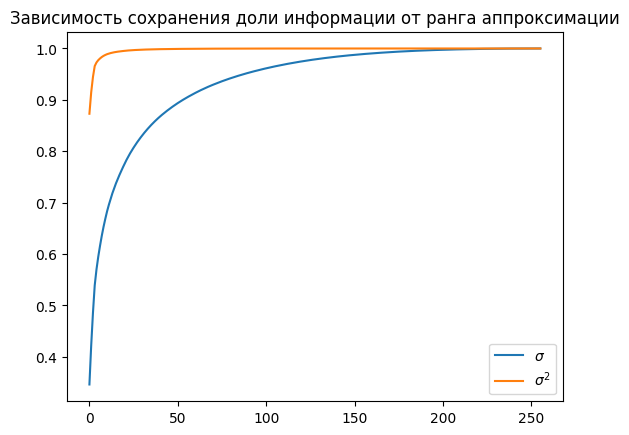
\includegraphics[width=1.0\textwidth]
    {images/solutions_analysis/svd/svd_lin_vs_square.png}
    \caption{Сравнение зависимости доли сохраняемой информации изображения от ранга приближения.}
    \label{fig:svd_lin_vs_square}
\end{figure}

Для более удобной настройки гиперпараметра $p$, будем вычислять ранг $k$ следующим образом:

$$
    \sum_{i=1}^{k} \sigma_i <= p\sum_{i=1}^{im\_size} \sigma_i < \sum_{i=1}^{k+1} \sigma_i,
$$

\subsubsection{Построение токенизатора на основе сингулярного разложения}

Для построения токенизатора изображений на основе сингулярного разложения будем использовать приближение изображения по динамическому рангу с линейной суммой сингулярных чисел.

Перепишем разложение матрицы $I_k$:

$$
I_k = U_k\Sigma_kV_k^T = (U_k\sqrt{\Sigma_k})(\sqrt{\Sigma}V_k^T) = U'V'^T
$$

Таким образом получаем матрицы $U'$ и $V'$. Для разбиения на исходной матрицы на набор векторов, разобьем матрицы $U'$ и $V'$ на наборы векторов $u_1, u_2, u_3, \cdots$ и $v_1, v_2, v_3, \cdots$, после чего попарно объединим вектора $u_i$ и $v_i$ в один вектор (выполним операцию конкатенации векторов).

Поскольку рассматривается токенизация трехканальных цветных изображений, то такое разбиение выполняется для каждого канала по отдельности. После чего полученные векторы объединяются в один.

$$
t = \text{concat}(u_{i1}, v_{i1}, u_{i2}, v_{i2}, u_{i3}, v_{i3}),
$$

где $\text{concat()}$ - операция конкатенации векторов, а $u_{i1}, v_{i1}, u_{i2}, v_{i2}, u_{i3}, v_{i3}$ - вектора, соответсвующие $i$-столбцам матриц $U'$ и $V'$ каждого из трех каналов исходного изображения.

Полученный набор векторов преобразуется с помощью линейного полносвязного слоя, слоя проекции, в размерность пространства токенов трансформера. При таком разбиении, исходный тензор размерности

$$
(3, M, M)
$$

преобразуется в последовательность токенов размерности

$$
(k, s_E)
$$

Стоит учесть, что поскольку ранг вычисляется динамически, то при обработке в программе одного минибатча для каждого изображения может быть вычислен различный ранг. В этом случае, выбирается максимальный ранг для всех изображений.

К полученной последовательности добавляется токен класса и позиционное кодирование, аналогичное используемому в модели Transformer.

\subsubsection{Результаты обучения}

Сначала было проведено сравнение обучения модели с токенизацией на основе сингулярного разложения с Vision Transformer. Для обучения был построен токенизатор на основе сингулярного разложения с использованием динамического ранга аппроксимации.

Результаты обучения и представлены в \autoref{tab:svd-tokenization}.

\begin{table}[H]
  \centering
  \begin{tabular}{|l|c|c|c|}
    \hline
    \makecell{Метод \\ токенизации} 
      & {Точность} 
      & {F1-метрика} 
      & \makecell{Средняя длина \\ входной последовательности} \\ 
    \hline
    Vision Transformer & 0.79 & 0.79 & 257 \\
    SVD-токенизация & 0.69 & 0.69 & 15.3 \\ \hline
  \end{tabular}
    \caption{Сравнение результатов обучения моделей с токенизатором на основе сингулярного разложения (SVD) с моделью Vision Transformer}
  \label{tab:svd-tokenization}
\end{table}

При обучении модели доля сохраненной информации токенизатором на основе сингулярного разложения была выбрана $p = 0.900$.

Из результатов, представленных в \autoref{tab:svd-tokenization}, видно, что метод токенизации на основе сингулярного разложения работоспособен. Причем, несмотря на небольшое падение значений метрик, удалось значительно сократить длину входной последовательности.

В \autoref{tab:svd-tokenization-disp} приведено сравнение результатов обучения модели с токенизатором на основе сингулярного разложения при различных значениях гиперпараметра доли сохраненной информации.

\begin{table}[H]
  \centering
  \begin{tabular}{|l|c|c|c|c|}
    \hline
    \makecell{Метод \\ токенизации}
      & \makecell{Доля \\ сохраненной \\ информации}
      & {Точность} 
      & {F1-метрика} 
      & \makecell{Средняя длина \\ входной \\ последовательности} \\ 
    \hline
    SVD-токенизация & 0.90 & 0.69 & 0.69 & 15.3 \\
    SVD-токенизация & 0.95 & 0.64 & 0.64 & 89.1 \\
    SVD-токенизация & 0.99 & 0.67 & 0.67 & 159.7 \\ \hline
  \end{tabular}
  
  \caption{Сравнение результатов обучения моделей с токенизатором на основе сингулярного разложения при разных значениях доли сохраненной информации}
  \label{tab:svd-tokenization-disp}
\end{table}

Получены контринтуитивные результаты, при которых большая доля сохранения информации приводит к падению метрик на этапе валидации. Вероятно, это вызвано тем, что большая динамическая длина последовательности приводит к ухудшению обучения модели.

\subsubsection{Проблемытокенизатора на основе сингулярного разложения}

Текущая версия токенизатора имеет следующие проблемы:

\begin{enumerate}
    \item Падение метрик даже при большой доли сохраненной информации.
    
        Несмотря на большую долю сохраненной информации и длину входной последовательности, полученные метрики оказались хуже. Это может свидетельствовать о том, что некоторые из компонент сингулярного разложения оказывают негативное влияние на результат работы нейронной сети.
    \item Требование к фиксированному размеру изображений.
    
        Поскольку в текущей версии токенизатора размерность изображения напрямую влияет на количество параметров токенизатора (на этапе линейной проекции), то возникает требование к фиксированному размеру изображений.
        
    \item Отсутствие оптимизации при вычислениях на графических ускорителях.
    
        Вычисление сингулярного выражения тяжело параллелизовать, из-за чего падает общая скорость обучения и работы модели. 
\end{enumerate}

Поскольку токенизатор на основе сингулярного разложения работоспособен и позволяет значительно сократить длину входной последовательности при обработке изображения, необходимо решить существующие проблемы для его эффективного обучения и использования.

\subsection{Модифицированный токенизатор на основе сингулярного разложения}

\subsubsection{Построение модифицированного токенизатора на основе сингулярного разложения без функции оценки}

Для решения проблем токенизатора на основе сингулярного разложения пришлось отказаться от использования сингулярного разложения. Алгоритм разложения был заменен на нейронную сеть, архитектура которой вдохновлена сингулярным разложением.

В алгоритме токенизации на основе сингулярного разложения, описанном в предыдущем разделе, токенизация происходит благодаря разбиению матриц $U'$ и $V'$ на наборы векторов $u$ и $v$. Для того, чтобы получить наборы векторов $u$ и $v$ с помощью нейронных сетей, воспользуемся алгоритмом пиксельной расстановки, аналогичным использованному в методе токенизации на основе быстрого преобразования Фурье. 

Для получения каждого из этих наборов построим нейронную сеть, принимающую на вход тензор размерности 

$$
(3, M, M)
$$

Данная нейронная сеть аналогична нейронной сети, предложенной в методе токенизации с использованием быстрого преобразования Фурье. Она также состоит из четырех блоков, каждый блок состоит из свёрточного слоя с размером ядра свёртки равным 3, размером шага равным 1, размером отступа равным 1 и с использованием нейрона смещения. Следом за свёрточным слоем используется слой нормализации и функция активации, после чего применяется алгоритм пиксельной расстановки. 

Таким образом, исходный тензор преобразуется в тензор размерности

$$
\Big(3 \cdot 4^4, \dfrac{M}{16}, \dfrac{M}{16}\Big)
$$

Данный тензор обрабатывается слоем проекции - свёрточным слоем с ядром свёртки размером 1, шагом свёртки размером 1, отступом размером 0 и без нейрона смещения. После этого, данный тензор выпрямляется по двум последним осям (``по ширине`` и ``по высоте``) и транспонируется. В результате получается тензор, описывающий последовательность векторов и имеющий размерность

$$
\Big(\dfrac{M^2}{16^2}, s_E\Big)
$$

Таким образом получаются наборы векторов $u$ и $v$. Аналогично методу токенизации на основе сингулярного разложения, два этих набора векторов объединяются в результате конкатенации соответствующих токенов. 

В результате получается тензор размерности

$$
\Big(\dfrac{M^2}{16^2}, 2 \cdot s_E\Big)
$$

Данный тензор с помощью линейного полносвязного слоя проецируется в пространство токенов трансформера. Итоговый тензор, описывающий последовательность токенов на вход трансформера, имеет размерность

$$
\Big(\dfrac{M^2}{16^2}, s_E\Big)
$$

Таким образом данная версия метода токенизации на основе сингулярного разложения позволяет решить проблему требования фиксированного размера изображения, поскольку динамическая переменная присутствует только в длине последовательности. Единственное требование к размеру изображения - кратность 16. Также, данная версия позволяет решить проблему отсутствия оптимизации вычисления на видеокарте, поскольку она полностью реализована с помощью слоёв нейронных сетей, оптимизированных для вычисления на графических ускорителях во всех популярных библиотеках глубокого обучения. 

Стоит отметить, что в отличие от исходного метода токенизации на основе сингулярного разложения, данный метод токенизации не выполняет фильтрацию токенов входной последовательности трансформера ни в каком виде. Из-за этого длина последовательности токенов, получаемой данным токенизатором при обработке изображения равна длине последовательности токенов, получаемом при использовании токенизатора Vision Transformer.

К итоговой последовательности токенов добавляется токен класса и позиционное кодирование, аналогичное позиционному кодированию в оригинальной модели Trasnformer.

Данная версия токенизатора названа mSVD. Общая схема представлена на \autoref{fig:msvd_scheme}.

\begin{figure}[H]
    \centering
    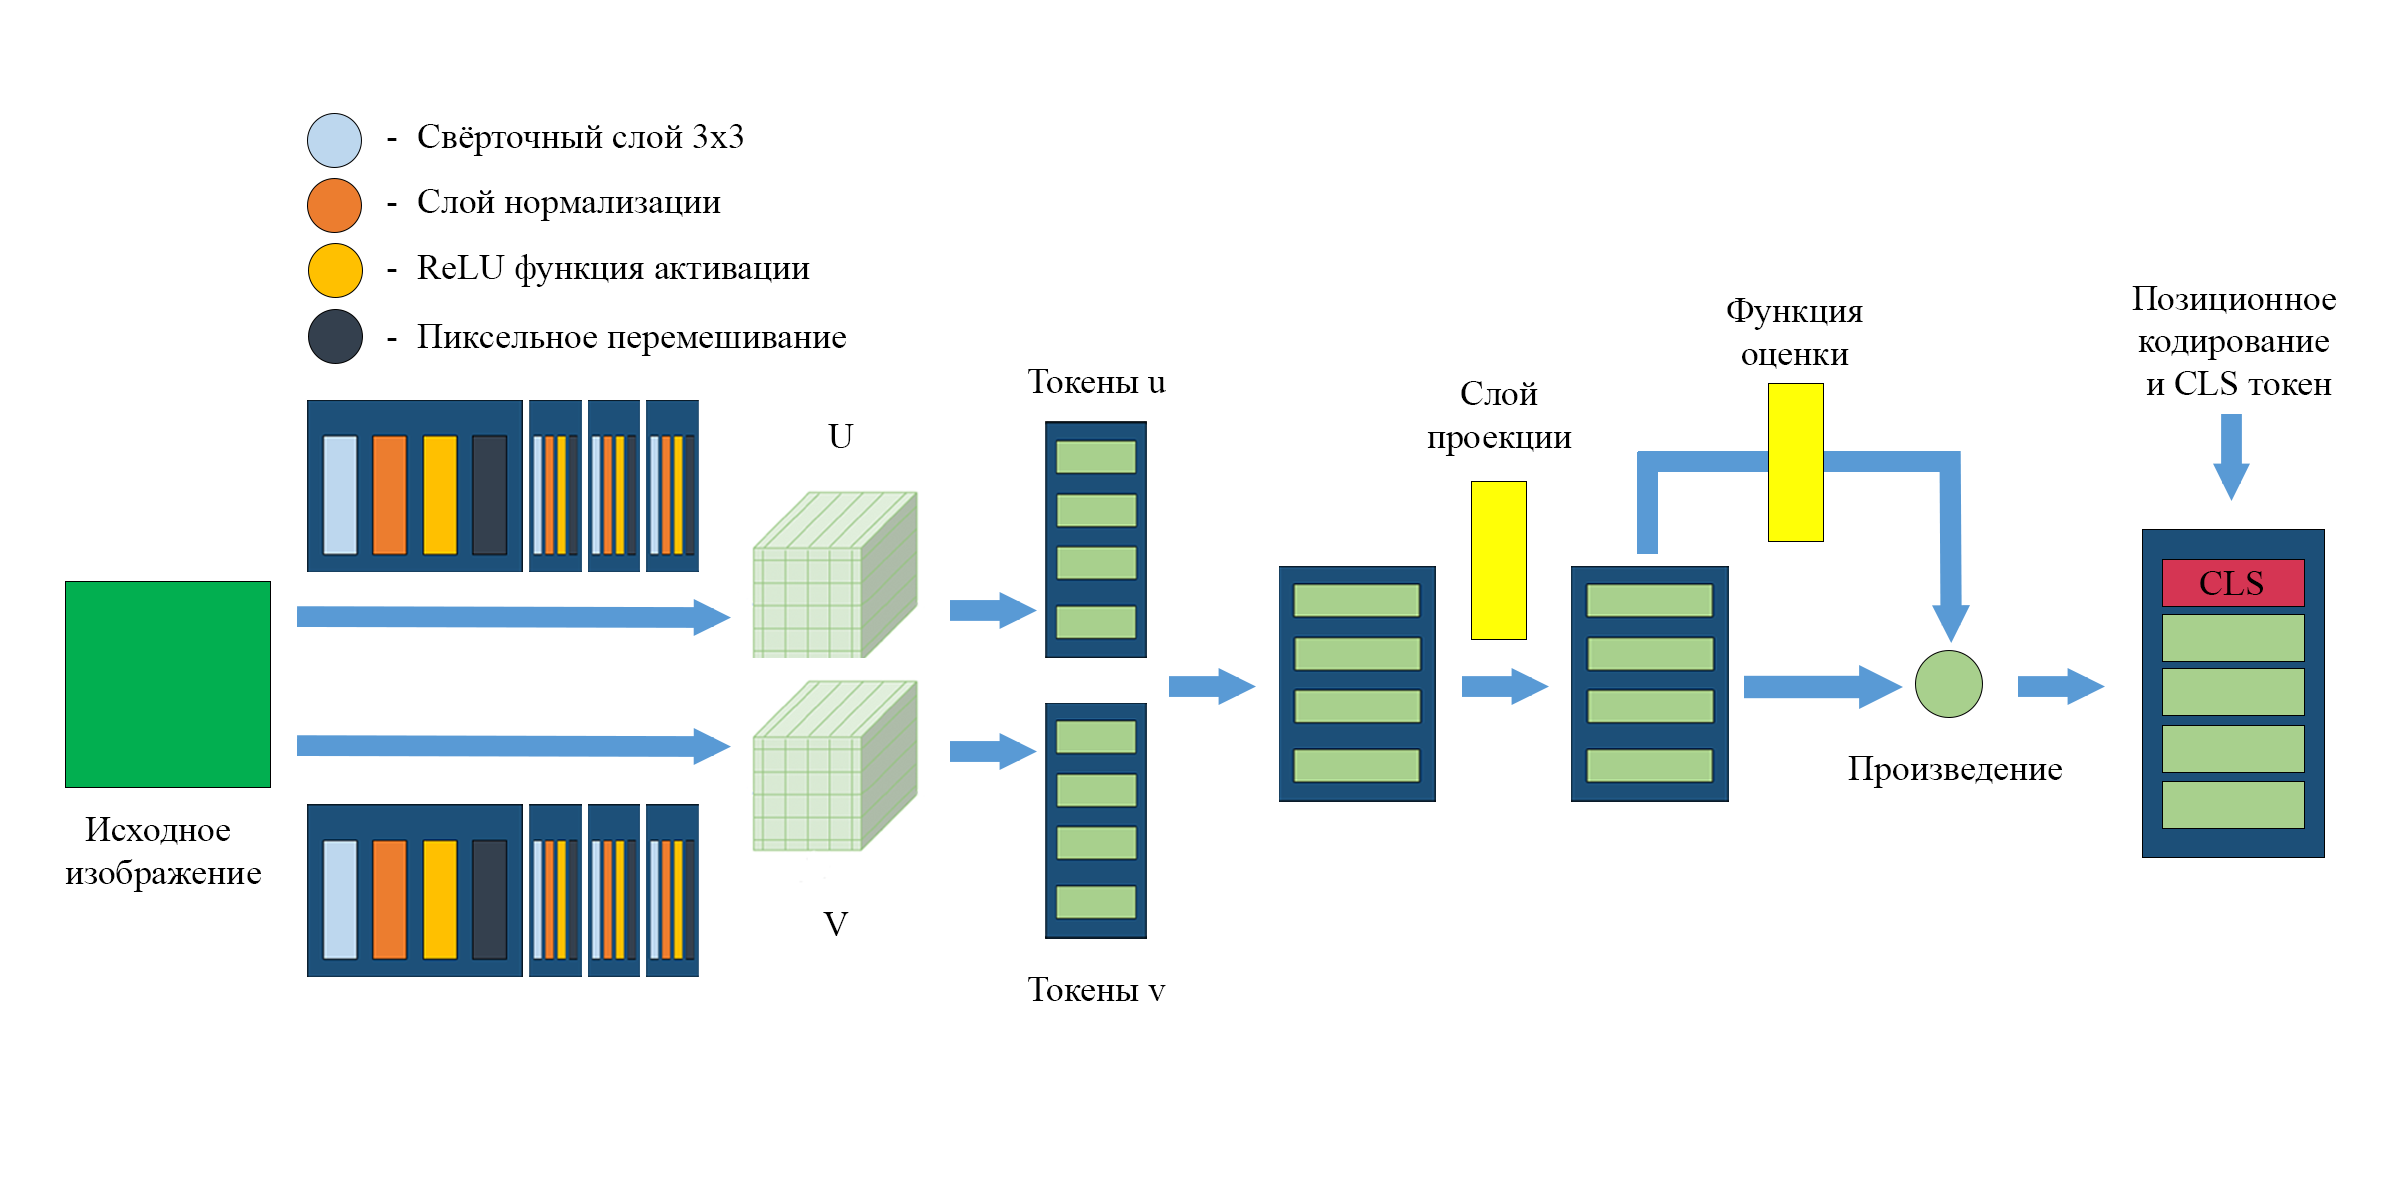
\includegraphics[width=1.0\textwidth]
    {images/research/msvd/msvd_scheme.png}
    \caption{Схема токенизатора mSVD.}
    \label{fig:msvd_scheme}
\end{figure}



\subsubsection{Построение функции оценки}
Для фильтрации токенов входной последовательности была добавлена функция оценки токенов. Функция оценки токенов формирует оценку ``важности`` токена. Данная функция реализована с помощью многослойной нейронной сети.

Для обучения функции оценки, вычисляемая оценка умножается на соотвествующий токен. Это позволяет градиентам при обучении достигать весов функции оценки. Однако, без дополнительных изменений, функция оценки будет выдавать одно и то же значение. Для эффективного обучения функции оценки необходим вспомогательная функция потерь.

Первая такая функция потерь была построена на основе индекса Джини \cite{gini}. Предполагая, что оценка токена - величина положительная, к выходу функции оценки применяется функция активации Rectified Linear Unit (ReLU). 

$$
\text{ReLU}(x) = \dfrac{x + |x|}{2}
$$

Если без обучения функция оценки дает одинаковые оценки всем токенам, то необходимо штрафовать нейроную сеть за одинаковые оценки. Для этого использована такая мера неоднородности, как индекс (коэффициент) Джини.

Коэффициент Джини для непрерывных элементов вычисляется следующим образом:

$$
G(x) = \dfrac{\sum\limits_{i=1}^n\sum\limits_{j=1}^n|x_i - x_j|}{2n^2\bar x}
$$

здесь $x_i$ - элемент последовательности, $n$ - длина последовательности, совпадает с количеством токенов, $\bar x$ - среднее значение элементов последовательности.

Поскольку $G(x) = 0$ при совпадении всех элементов последовательности $x$, то функция потерь, основанная на индексе Джини, выглядит следующим образом:

$$
L_G(x) = \beta(1 - G(x)),
$$

где $\beta$ - коэффициент вспомогательной функции потерь.

Также был рассмотрен иной метод построения функции потерь, основанный на идее регуляризации.

Выход функции оценки обрабатывается с помощью функции активации сигмоида

$$
\sigma(x) = \dfrac{1}{1 + e^{-x}}
$$

Полученные после обработки результаты назовём шлюзами $g_i = \sigma(x_i)$. Шлюзы могут принимать значения от 0 до 1. Для обучения функции оценки, каждый токен последовательности умножается на соответствующий ему шлюз. Это позволяет градиентам при обучении доходить до функции оценки. 

В случае, если значение шлюза близко к нулю, то после умножения на него, соответствующий токен становится близок к нулю и оказывает меньшее влияние на результат предсказания нейронной сети. В случае, если значения шлюза близко к единице, то соответствующий токен почти не изменяется при обучении.

Для того, чтобы функция оценок не обучилась таким образом, чтобы ``пропускать`` все токены (то есть предсказывать все значения шлюзов близкими к единице), в качестве вспомогательного лосса используется регуляризация шлюзов:

$$
L_g = \alpha \dfrac{1}{n}\sum_{i=1}^n g_i,
$$

где $\alpha$ - коэффициент вспомогательной функции потерь.

\subsubsection{Метод фильтрации токенов}
После получения оценок выполняется фильтрация токенов. Подобно предыдущим методам, можно выделить статический метод фильтрации и динамический.

Статический метод фильтрации заключается в отборе $k$ лучших токенов по их оценкам. В этом случае после добавления позиционного кодирования к последовательности токенов изначальной длины, по оценкам отбираются $k$ лучших токенов. Таким образом, длина новой последовательности равна $k$.

Динамический метод фильтрации заключается в вычислении суммы оценок токенов (или шлюзов) и отборе наименьшего количества токенов, сумма оценок которых не меньше доли $p$ от общей суммы оценок. В случае, если в одном минибатче получаются различные значения длины последовательности, из них выбирается максимальная.

Благодаря наличию функции оценки токенов, при обучении нейронной сети с методом mSVD-токенизации можно не использовать фильтрацию. При этом во время работы нейронной сети в режиме предсказания, можно изменять гиперпараметры применяемых методов фильтрации. Так, для одного избражения возможно применение статического метода фильтрации, а для другого - динамического без необходимости переобучения исходной нейронной сети.


\subsubsection{Результаты обучения}

Сначала было проведено обучение модели с mSVD токенизатором без функции оценки для проверки и демонстрации ее работоспособности.

При обучении модели с рассматриваемым токенизатором (mSVD) без функции оценки и фильтрации токенов, размер последовательности токенов совпадает с размером последовательности при использовании токенизации Vision Transformer с размером патча 16. 

Результаты обучения представлены в \autoref{tab:msvd-tokenization-no-scorer}:

\begin{table}[H]
  \centering
  \begin{tabular}{|l|c|c|c|}
    \hline
    \makecell{Метод \\ токенизации} 
      & {Точность} 
      & {F1-метрика} 
      & \makecell{Длина \\ входной \\ последовательности} \\ 
    \hline
    \makecell{Vision Transformer} & 0.79 & 0.79 & 257 \\
    \makecell{mSVD} & 0.85 & 0.85 & 257 \\ \hline
  \end{tabular}
    \caption{Сравнение результатов обучения моделей с использованием mSVD-токенизатора и модели Vision Transformerr}
  \label{tab:msvd-tokenization-no-scorer}
\end{table}

При использовании данного метода токенизации получается достигнуть более высоких значений метрик, уменьшив количество неверно определенных классов на четверть.

Далее было проведено обучение модели с mSVD токенизатором cо вспомогательной функцией потерь на основе индекса Джини при разных значениях коэффициента $\beta$. Для фильтрации токенов использовался динамический метод фильтрации при доле $p=0.900$.

Результаты обучения представлены в \autoref{tab:msvd-tokenization-gini}.

\begin{table}[H]
  \centering
  \begin{tabular}{|l|c|c|c|}
    \hline
    \makecell{Метод \\ токенизации} 
      & {Точность} 
      & {F1-метрика} 
      & \makecell{Средняя \\ длина входной \\ последовательности} \\ 
    \hline
    \makecell{Vision Transformer} & 0.79 & 0.79 & 257 \\
    \makecell{mSVD} & 0.85 & 0.85 & 257 \\ 
    \makecell{mSVD (Джини, $\beta=1.0$)} & 0.82 & 0.82 & 231.4 \\
    \makecell{mSVD (Джини, $\beta=0.5$)} & 0.82 & 0.82 & 231.3 \\
    \makecell{mSVD (Джини, $\beta=0.1$)} & 0.82 & 0.82 & 231.3 \\
    \hline
  \end{tabular}
    \caption{Сравнение результатов обучения моделей с использованием mSVD-токенизатора при вспомогательной функции потерь на основе коэффициента Джини и модели Vision Transformer.}
  \label{tab:msvd-tokenization-gini}
\end{table}

Получены одинаковые результаты для разных значений параметра $\alpha$. Это означает, что вспомогательная функция потерь на основе коэффициента Джини не оказывает никакого влияния на результат обучения модели. 

Также, об этом может свидетельствовать средняя длина входной последовательности. Можно заметить, что $231.4 = p \cdot 256 + 1$. Таким образом, функция оценки дает приблизительно одинаковые значения для любых токенов последовательности. Это означает, что функция потерь на основе индекса Джини неработоспособна.

Несмотря на это, стоит заметить, что итоговая модель все равно превосходит по значениям метрик Vision Transformer, имея при этом меньшую длину входной последовательности на десятую часть.

Поскольку функция потерь на основе индекса Джини оказалась неработоспособна, было проведено обучение модели с mSVD токенизатором cо вспомогательной функцией потерь на основе регуляризации шлюзов.

Фильтрация токенов отсутствует, результаты обучения представлены в \autoref{tab:msvd-tokenization-sigmoid-gating}:

\begin{table}[H]
  \centering
  \begin{tabular}{|l|c|c|c|}
    \hline
    \makecell{Метод \\ токенизации} 
      & {Точность} 
      & {F1-метрика} 
      & \makecell{Длина \\ входной \\ последовательности} \\ 
    \hline
    \makecell{Vision Transformer} & 0.79 & 0.79 & 257 \\
    \makecell{mSVD} & 0.85 & 0.85 & 257 \\ 
    \makecell{mSVD ($\alpha = 0.0250$)} & 0.83 & 0.83 & 257 \\ 
    \makecell{mSVD ($\alpha = 0.0125$)} & 0.85 & 0.85 & 257 \\
    \makecell{mSVD ($\alpha = 0.0050$)} & 0.85 & 0.84 & 257 \\
    \hline
  \end{tabular}
    \caption{Сравнение результатов обучения моделей с использованием mSVD-токенизатора при вспомогательной функции потерь на основе регуляризации шлюзов и модели Vision Transformer}
  \label{tab:msvd-tokenization-sigmoid-gating}
\end{table}

Лучшие результаты обучения были получены при значении $\alpha = 0.0125$. По результатам этого эксперимента, данное значение параметра выбирается по умолчанию для всех последующих экспериментов. 

Можно заметить, что лучшие значения метрик при обучении рассматриваемого метода токенизации с использованием функции оценки не превосходят значения метрик при обучении метода токенизации без использования функции оценки. Это ожидаемый результат, поскольку функция оценки никак не добавляет дополнительной информации при обработке изображения.

Далее, было также проведено сравнение статического и динамического методов фильтрации токенов.

Результаты обучения представлены в \autoref{tab:msvd-tokenization-static-dynamic}:

\begin{table}[H]
  \centering
  \begin{tabular}{|l|c|c|c|}
    \hline
    \makecell{Метод \\ токенизации} 
      & {Точность} 
      & {F1-метрика} 
      & \makecell{Средняя \\ длина входной \\ последовательности} \\ 
    \hline
    \makecell{Vision Transformer} & 0.79 & 0.79 & 257 \\
    \makecell{mSVD} & 0.85 & 0.85 & 257 \\ 
    \hline
    \makecell{mSVD (k=1)} & 0.43 & 0.40 & 2 \\ 
    \makecell{mSVD (k=4)} & 0.52 & 0.48 & 5 \\
    \makecell{mSVD (k=16)} & 0.61 & 0.57 & 17 \\
    \makecell{mSVD (k=32)} & 0.66 & 0.63 & 33 \\
    \makecell{mSVD (k=64)} & 0.71 & 0.70 & 65 \\
    \makecell{mSVD (k=96)} & 0.76 & 0.75 & 97 \\
    \makecell{mSVD (k=128)} & 0.80 & 0.80 & 129 \\
    \makecell{mSVD (k=160)} & 0.83 & 0.83 & 161 \\
    \makecell{mSVD (k=192)} & 0.85 & 0.85 & 193 \\
    \makecell{mSVD (k=224)} & 0.85 & 0.85 & 225 \\
    \hline
    \makecell{mSVD (p=0.100)} & 0.62 & 0.58 & 23.1 \\
    \makecell{mSVD (p=0.200)} & 0.67 & 0.64 & 46.6 \\
    \makecell{mSVD (p=0.300)} & 0.71 & 0.69 & 70.0 \\
    \makecell{mSVD (p=0.400)} & 0.74 & 0.73 & 90.4 \\
    \makecell{mSVD (p=0.500)} & 0.77 & 0.77 & 120.2 \\
    \makecell{mSVD (p=0.600)} & 0.81 & 0.81 & 149.4 \\
    \makecell{mSVD (p=0.700)} & 0.83 & 0.83 & 166.0 \\
    \makecell{mSVD (p=0.800)} & 0.85 & 0.85 & 192.5 \\
    \makecell{mSVD (p=0.900)} & 0.85 & 0.85 & 228.9 \\
    \makecell{mSVD (p=0.950)} & 0.85 & 0.85 & 242.2 \\
    \makecell{mSVD (p=0.990)} & 0.85 & 0.85 & 253.6 \\
    \hline
  \end{tabular}
    \caption{Сравнение статического и динамического методов фильтрации токенов}
  \label{tab:msvd-tokenization-static-dynamic}
\end{table}

Видно, что с помощью методов фильтрации на основе оценок токенов возможно сократить длину последовательности на четверть и не потерять в качестве работы модели. При этом, если сократить длину последовательности в два раза, то значения метрик все равно будут выше, чем при использовании Vision Transformer.

\subsection{Сравнение предложенных алгоритмов токенизации изображений и существующих решений}
\subsubsection{Токенизация изображений на основе Вейвлет-преобразования}
В работе \cite{wavelet_autoregression}, где предложен метод токенизации изображений на основе Вейвлет-преобразования, основная цель метода - авторегрессионная генерация изображения. Однако, данный метод может быть адаптирован и для других задач, связанных с обработкой изображений. Например, для решения задачи многоклассовой классификации.

Однако, применить данный метод для обработки изображений размерности больше, чем (3, 32, 32) не вышло, поскольку длина последовательности токенов становится равной нескольким тысячам. Это приводит к серьезной нехватке памяти и значительно снижает скорость обработки данных.

\subsubsection{Результаты обучения и сравнение с предложенными методами}

Лучшие результаты по всем рассмотренным методам были сведены в единую таблицу (\autoref{tab:research-comparison}). В качестве FFT-токенизатора выбран токенизатор с размером статического фильтра 256, в качестве SVD-токенизатора выбран токенизатор с долей сохраненной информации равной 0.90, в качестве mSVD токенизатора был выбран токенизатор с динамической фильтрацией токенов с долей от суммы оценок равной 0.800.

\begin{table}[H]
  \centering
  \begin{tabular}{|l|c|c|c|}
    \hline
    \makecell{Метод \\ токенизации} 
      & {Точность} 
      & {F1-метрика} 
      & \makecell{Средняя \\ длина входной \\ последовательности} \\ 
    \hline
    \makecell{Vision Transformer} & 0.79 & 0.79 & 257 \\
    \makecell{Вейвлет-токенизатор} & 0.50 & 0.43 & 1025 \\
    \makecell{FFT-токенизатор} & 0.79 & 0.79 & 257 \\
    \makecell{SVD-токенизатор} & 0.69 & 0.69 & 15.3 \\
    \makecell{mSVD} & 0.85 & 0.85 & 192.5 \\ 
    \hline
  \end{tabular}
    \caption{Сравнение построенных токенизаторов с токенизатором на основе Вейвлет-преобразования и Vision Transformer}
  \label{tab:research-comparison}
\end{table}


Из \autoref{tab:research-comparison} видно, что лучшие результаты были получены при использовании модели с токенизатором mSVD.

\subsection{Выводы по главе 3}

В результате исследования алгоритмов токенизации изображений на основе матричных разложений были построены рабочие методы токенизации на основе быстрого преобразования Фурье и сингулярного разложения. Однако, данные методы обладают серьезными недостатками, такими как ухудшение качества работы итоговой модели по сравнению с Vision Transformer и медленное вычисление матричных разложений, не оптимизированных для работы на видеокартах. 

Попытка решить эти недостатки привела к созданию метода токенизации mSVD, сохранившего преимущества Vision Transformer, такие как возможность параллельного вычисления и возможность обработки, и добившегося более высокой точности работы итоговой модели при меньшей длине входной последовательности. 


\newpage
\documentclass[times,specification,annotation]{itmo-student-thesis}
\usepackage{fancyhdr}

%% Опции пакета:
%% - specification - если есть, генерируется задание, иначе не генерируется
%% - annotation - если есть, генерируется аннотация, иначе не генерируется
%% - times - делает все шрифтом Times New Roman, собирается с помощью xelatex
%% - languages={...} - устанавливает перечень используемых языков. По умолчанию это {english,russian}.
%%                     Последний из языков определяет текст основного документа.

%% Делает запятую в формулах более интеллектуальной, например:
%% $1,5x$ будет читаться как полтора икса, а не один запятая пять иксов.
%% Однако если написать $1, 5x$, то все будет как прежде.
\usepackage{icomma}

%% Один из пакетов, позволяющий делать таблицы на всю ширину текста.
\usepackage{tabularx}

%% Данные пакеты необязательны к использованию в бакалаврских/магистерских
%% Они нужны для иллюстративных целей
%% Начало
\usepackage{tikz}
\usetikzlibrary{arrows}
\usepackage{filecontents}
%% Конец

%% Указываем файл с библиографией.
\addbibresource{bachelor-thesis.bib}


\begin{document}

\chapter{Использование предложенных алгоритмов токенизации изображений для решения различных нейросетевых задач обработки изображений}

\section{Решение задачи регрессии}

\subsection{Решение задачи регрессии моделью с токенизатором, основанным на быстром преобразовании Фурье}


\subsection{Решение задачи регрессии моделью с токенизатором mSVD}


\section{Генерация изображений с использованием предложенных методов токенизации}

\subsection{Использование алгоритма токенизации, основанного на быстром преобразовании Фурье}


\subsection{Использование алгоритма токенизации mSVD}

% Старый текст


Детокенизатор mSVD строится как отраженная копия токенизатора mSVD. В начале, набор векторов размерности

$$
\Big(\dfrac{M^2}{16^2}, s_E\Big)
$$

преобразуется в тензор размерности

$$
\Big(s_E, \dfrac{M}{16}, \dfrac{M}{16}\Big)
$$

Следом, полученный тензор обрабатывается последовательность алгоритмов пиксельных перемешиваний, функций активации и свёрточных слоёв c размером ядра свёртки 3, шагом 1, отступом 1 и с нейроном смещения. Однако, поскольку в mSVD токенизаторе присутстовало две ветви нейронных сетей, ответственных за получение наборов векторов $u$ и $v$ соответственно, то для поддержания симметрии токенизатора и детокенизатора, вместо одного свёрточного слоя на один этап пиксельного перемешивания, используется 2 свёрточных слоя.

Таким образом, детокенизатор mSVD имеет 4 блока, состоящих из свёрточного слоя, нормализации, функции активации, свёрточного слоя, нормализации, функции активации и пиксельного перемешивания.

Полученный после преобразования тензор имеет размерность 

$$
\Big(\dfrac{s_E}{16^2},  M, M\Big)
$$

Данный тензор проецируется в трехканальное изображение с помощью слоя проекции. Данный слой представлен в виде свёрточного слоя с размером ядра свёртки 1, шагом свёртки 1, размером отступа 0 и без нейрона смещения.






\subsection{Авторегрессионная генерация изображений с использованием mSVD-токенизатора}

Для решения задачи авторегрессионной генерации вдохновимся идеями, предложенными в работе DALLE. Так, представим токенизатор как модель-кодировщик, задача которой - закодировать изображение в набор векторов. В работе, посвященной DALLE, используется дискретный вариационный автокодировщик. Поскольку трансформер работает только с наборами векторов, то после обработки закодированного набора векторов трансформером, для восстановления изображения потребуется детокенизатор.


%\subsection{Обучение токенизатора и детокинезатора для авторегрессионной генерации изображений}


%\subsection{Обучение трансформера для авторегрессионной генерации изображений с использованием токинезатора и детокинезатора mSVD}

% \chapterconclusion

\end{document}

\newpage
\section*{Заключение}
\addcontentsline{toc}{section}{Заключение}

В результате выполненного исследования разработаны и оценены новые методы токенизации изображений на основе матричных разложений, которые решают ряд ограничений классичесского подхода Vision Transformer. Поставленные цели работы были достигнуты.
\newpage

\addcontentsline{toc}{section}{Список использованных источников}

\section*{Список использованных источников}
\printbibliography[heading=none]

\newpage
\appendix
\section*{Приложение А\\Код модели токенизатора на основе быстрого преобразования Фурье}
\addcontentsline{toc}{section}{Приложение А. Код модели токенизатора на основе быстрого преобразования Фурье}

\noindent Листинг А.1 — Python-код низкочастотного фильтра
{\scriptsize
\begin{verbatim}
class FFTLowFreqFilter(nn.Module):
    def __init__(
        self,
        filter_size: int = 0,
        energy_ratio: float = 0.9,
        downscale_factors = None,
        eps: float = 1e-8
    ):
        super().__init__()
        self.filter_size = filter_size
        self.energy_ratio = energy_ratio

        self.downscale_factors = downscale_factors or []
        self.total_downscale = math.prod(self.downscale_factors)
        self.eps = eps


    def compute_filter_size(self, power: torch.Tensor):
        B, W, H = power.shape
        cumsum_h = torch.cumsum(power, dim=1)        # [B, W, H]
        integral = torch.cumsum(cumsum_h, dim=2)     # [B, W, H]
        total_energy = integral[:, -1, -1]           # [B]
        max_k = min(W, H)
        cx, cy = W // 2, H // 2

        for fs in range(self.total_downscale, max_k + 1, self.total_downscale):
            half = fs // 2
            x0, y0 = cx - half, cy - half
            x1, y1 = x0 + fs, y0 + fs

            A = integral[:, x1-1, y1-1]
            B_ = integral[:, x0-1, y1-1] if x0 > 0 else 0
            C = integral[:, x1-1, y0-1] if y0 > 0 else 0
            D = integral[:, x0-1, y0-1] if x0 > 0 and y0 > 0 else 0
            low_energy = A - B_ - C + D  # [B]
            if torch.all(low_energy / (total_energy + self.eps) >= self.energy_ratio):
                return fs

        return (max_k // self.total_downscale) * self.total_downscale or self.total_downscale

    def forward(self, x: torch.Tensor):
        F = fft.fft2(x, norm='ortho')              # [B, 3, W, H]
        F = fft.fftshift(F, dim=(-2, -1))
        real, imag = F.real, F.imag

        signed_log = lambda v: torch.sign(v) * torch.log1p(v.abs() + self.eps)
        log_real = signed_log(real)
        log_imag = signed_log(imag)

        fs = self.filter_size
        if fs == 0:
            power_spectrum = log_real.pow(2) + log_imag.pow(2)      # [B, 3, W, H]
            energy = power_spectrum.sum(dim=1)              # [B, W, H]
            fs = self.compute_filter_size(energy)

        freq_cat = torch.cat([log_real, log_imag], dim=1)  # [B, 6, W, H]

        B, C, W, H = freq_cat.shape
        half = fs // 2
        cx, cy = W // 2, H // 2
        x0, y0 = cx - half, cy - half
        low_freq = freq_cat[:, :, x0:x0 + fs, y0:y0 + fs]

        return {"tensor": low_freq, "filter_size": fs}

\end{verbatim}
}

\noindent Листинг А.2 — Python-код модели токенизатора на основе быстрого преобразования Фурье
{\scriptsize
\begin{verbatim}

class MFFTTokenizer(nn.Module):
    def __init__(
        self,
        in_channels: int = 3,
        pixel_unshuffle_scale_factors: List[int] = [2, 2, 2, 2],
        embedding_dim: int = 768,
        filter_size: int = 0,
        energy_ratio: float = 0.9
    ):
        super().__init__()

        self.low_freq_filter = FFTLowFreqFilter(
            filter_size=filter_size,
            energy_ratio=energy_ratio,
            downscale_factors=pixel_unshuffle_scale_factors
        )
        self.in_channels = in_channels
        self.pixel_unshuffle_scale_factors = pixel_unshuffle_scale_factors
        self.embedding_dim = embedding_dim

        layers = []
        current_channels = in_channels * 2
        for scale in self.pixel_unshuffle_scale_factors:
            layers += [
                nn.Conv2d(current_channels, current_channels, kernel_size=3, padding=1),
                nn.BatchNorm2d(current_channels),
                nn.LeakyReLU(),
                nn.PixelUnshuffle(downscale_factor=scale)
            ]
            current_channels *= scale ** 2
        self.feature_extractor = nn.Sequential(*layers)

        self.linear_projection = nn.Linear(current_channels, embedding_dim)
        self.cls_token = nn.Parameter(torch.randn(1, 1, embedding_dim))
        self.positional_encoding = PositionalEncoding(embedding_dim)

    def _add_cls_token(self, tokens: torch.Tensor) -> torch.Tensor:
        cls = self.cls_token.to(tokens.device).expand(tokens.size(0), -1, -1)
        return torch.cat([cls, tokens], dim=1)

    def _add_positional_encoding(self, tokens: torch.Tensor) -> torch.Tensor:
        return tokens + self.positional_encoding(tokens)

    def forward(self, x: torch.Tensor) -> Dict[str, Any]:
        low = self.low_freq_filter(x)
        low_x, fs = low["tensor"], low["filter_size"]

        feat = self.feature_extractor(low_x)
        feat = feat.permute(0, 2, 3, 1).contiguous()

        B, H, W, C = feat.shape
        tokens = feat.view(B, H * W, C)
        tokens = self.linear_projection(tokens)
        tokens = self._add_cls_token(tokens)
        tokens = self._add_positional_encoding(tokens)

        return {"tokens": tokens, "filter_size": fs}
\end{verbatim}
}
\newpage
\appendix
\section*{Приложение B\\Код модели токенизатора на основе сингулярного разложения}
\addcontentsline{toc}{section}{Приложение B. Код модели токенизатора на основе сингулярного разложения}

\noindent Листинг B.1 — Python-код модели токенизатора на основе сингулярного разложения
{\scriptsize
\begin{verbatim}

class MSVDNoScorerTokenizer(nn.Module):
    def __init__(
            self,
            in_channels=3,
            pixel_unshuffle_scale_factors=[2, 2, 2, 2],
            dispersion=0.9,
            embedding_dim=768
    ):
        super().__init__()

        self.in_channels = in_channels
        self.pixel_unshuffle_scale_factors = pixel_unshuffle_scale_factors
        self.dispersion=dispersion

        self.u_feature_extractor = nn.ModuleList()
        current_channels = self.in_channels
        for scale in self.pixel_unshuffle_scale_factors:
            self.u_feature_extractor.append(
                nn.Conv2d(
                    in_channels=current_channels,
                    out_channels=current_channels,
                    kernel_size=3, padding=1, stride=1
                ),
            )
            self.u_feature_extractor.append(nn.BatchNorm2d(current_channels))
            self.u_feature_extractor.append(nn.LeakyReLU())
            self.u_feature_extractor.append(nn.PixelUnshuffle(downscale_factor=scale))
            current_channels = current_channels * (scale ** 2)
        self.u_feature_extractor = nn.Sequential(*self.u_feature_extractor)

        self.v_feature_extractor = nn.ModuleList()
        current_channels = self.in_channels
        for scale in self.pixel_unshuffle_scale_factors:
            self.v_feature_extractor.append(
                nn.Conv2d(
                    in_channels=current_channels,
                    out_channels=current_channels,
                    kernel_size=3, padding=1, stride=1
                )
            )
            self.v_feature_extractor.append(nn.BatchNorm2d(current_channels))
            self.v_feature_extractor.append(nn.LeakyReLU())
            self.v_feature_extractor.append(nn.PixelUnshuffle(downscale_factor=scale))
            current_channels = current_channels * (scale ** 2)
        self.v_feature_extractor = nn.Sequential(*self.v_feature_extractor)

        self.linear_projection = nn.Linear(
            in_features=current_channels * 2,
            out_features=embedding_dim
        )

        self.cls_token = nn.Parameter(torch.randn(1, 1, embedding_dim))
        self.positional_encoding = PositionalEncoding(embedding_dim)


    def _get_raw_tokens(self, x):
        raw_u = self.u_feature_extractor(x)
        raw_v = self.v_feature_extractor(x)

        raw_u = raw_u.permute(0, 2, 3, 1).contiguous()
        raw_v = raw_v.permute(0, 2, 3, 1).contiguous()

        B, H, W, C = projected_u.shape
        tokens_u = torch.reshape(raw_u, (B, H * W, C))
        tokens_v = torch.reshape(raw_v, (B, H * W, C))

        raw_tokens = torch.cat([tokens_u, tokens_v], dim=-1)
        return raw_tokens

    def _add_cls_token(self, tokens):
        batch_size = tokens.shape[0]
        cls_token = self.cls_token.expand(batch_size, -1, -1)
        tokens = torch.cat([cls_token, tokens], dim=1)
        return tokens

    def _add_positional_encoding(self, tokens):
        positional_encoding = self.positional_encoding(tokens)
        tokens = tokens + positional_encoding
        return tokens

    def _filter_tokens(self, sorted_weighted_tokens, sorted_sigmas):
        batch_size, n_tokens, raw_tokens_dim = sorted_weighted_tokens.shape

        sorted_sigmas_squeezed = sorted_sigmas.squeeze(dim=-1)
        sigma_sum = sorted_sigmas_squeezed.sum(dim=1, keepdim=True)
        threshold = self.dispersion * sigma_sum.unsqueeze(-1)

        cumsum_sigma = sorted_sigmas.cumsum(dim=1)
        keep_mask = cumsum_sigma <= threshold

        lengths = keep_mask.sum(dim=1)

        max_len = lengths.max().item()
        padded = sorted_weighted_tokens.new_zeros(batch_size, max_len, raw_tokens_dim)
        for b in range(batch_size):
            L = lengths[b]
            padded[b, :L] = sorted_weighted_tokens[b, :L]
        return padded, lengths

    def forward(self, x):
        raw_tokens = self._get_raw_tokens(x)

        tokens = self.linear_projection(raw_tokens)
        tokens = self._add_cls_token(tokens)
        tokens = self._add_positional_encoding(tokens)

        return tokens


\end{verbatim}
}

\noindent Листинг B.2 — Python-код модели токенизатора mSVD с функцией оценки токенов
{\scriptsize
\begin{verbatim}

class MSVDSigmoidGatingViT(nn.Module):
    def __init__(
            self,
            num_channels: int = 3,
            pixel_unshuffle_scale_factors: list = [2, 2, 2, 2],
            embedding_dim: int = 768,
            selection_mode: str = "full",
            top_k: int = 25,
            dispersion: float = 0.900,
            qkv_dim: int = 64,
            mlp_hidden_size: int = 1024,
            n_layers: int = 12,
            n_heads: int = 12,
            n_classes: int = 1000,
    ):
        super().__init__()

        self.tokenizer = MSVDSigmoidGatingTokenizer(
            in_channels=num_channels,
            pixel_unshuffle_scale_factors=pixel_unshuffle_scale_factors,
            embedding_dim=embedding_dim,
            selection_mode=selection_mode,
            dispersion=dispersion,
            top_k=top_k
        )

        self.transformer_encoder = TransformerEncoder(
            embed_dim=embedding_dim,
            qkv_dim=qkv_dim,
            mlp_hidden_size=mlp_hidden_size,
            n_layers=n_layers,
            n_heads=n_heads
        )

        self.classifier = nn.Sequential(
            nn.Linear(embedding_dim, 128),
            nn.ReLU(),
            nn.Linear(128, n_classes)
        )

    def forward(self, tensor):
        msvd_output = self.tokenizer(tensor)
        tokens = msvd_output["tokens"]
        scores = msvd_output["scores"]
        x = self.transformer_encoder(tokens)
        x = x[:, 0]
        logits = self.classifier(x)
        return {"logits": logits, "scores": scores}


\end{verbatim}
}

\end{document}